\documentclass[12pt,a4paper]{report}

\usepackage[T1]{fontenc}
\usepackage[utf8]{inputenc}
\usepackage[italian, shorthands=off]{babel} % Without shorthands=off, there is interference with hyperref package for footnotes
\usepackage{times} % Selected font
\usepackage[table, svgnames]{xcolor} % Colors
\usepackage{url} % To put URLs
\usepackage{xurl} % Avoids URLs to overfull \hbox
\usepackage{float} % For anchor options
\usepackage{graphicx} % Images
\graphicspath{{img/}}
\newcounter{figcounter} % Initialize new counter to 0
\usepackage{setspace} % For flexible line spacing management
\usepackage[margin=1in]{geometry} % Page geom
\usepackage{fancyhdr} % To define a custom page numbering style
\setlength{\headheight}{14.49998pt} % Avoids fancyhdr Warning, due to 12pt titles
\usepackage{csquotes} % Recommended package to load before biblatex
\usepackage[backend=biber, style=alphabetic, sorting=ydnt]{biblatex} % To include bibliography
\addbibresource{riferimenti.bib}
\usepackage{amsmath} % Necessary for \text{} command inside maths notations
\usepackage{bm} % Import the bm package, for bold math expressions
\usepackage{parskip} % Avoids paragraph indentation and puts spacing instead, better than the following two
% \setlength{\parskip}{0.5em} % Set global paragraph spacing
% \setlength{\parindent}{0pt} % No paragraph indentation
\usepackage{enumitem} % To avoid interline between bullets and text before them
\setlist[itemize]{topsep=0pt, partopsep=0pt, parsep=0pt}
\usepackage{subcaption} % For multiple graphs in a single picture
\usepackage{tikz} % To draw graphs
\usepackage{pgfplots} % To plot inside a graph in 2D
\pgfplotsset{compat=1.18} % Avoids pgfplots Warning
\usetikzlibrary{3d} % For 3D graphs
\usepackage{listings} % To use listings
% \usepackage{inconsolata} % Use Inconsolata
\renewcommand{\lstlistingname}{Listato} % Configurazione italiana del listato
\usepackage{tabularray} % For tables

\usepackage[colorlinks=true, linkcolor=blue, citecolor=blue, urlcolor=blue, pdfborder={0 0 0}, hyperfootnotes=true]{hyperref}
% You must include hyperref before hypcap
\usepackage[table, figure]{hypcap} % Ensures that references go to the figure or the table and not the caption

\definecolor{C_comment_green}{rgb}{0.0, 0.5, 0.0}
\definecolor{C_types_blue}{RGB}{30, 60, 240}
\definecolor{C_macro_blue}{RGB}{30, 105, 235}
\definecolor{C_enum_blue}{RGB}{30, 130, 210}
\definecolor{C_user_types_green}{RGB}{50, 222, 156}
\definecolor{C_directives_purple}{RGB}{140, 10, 133}
\definecolor{C_function_amber}{RGB}{200, 180, 20}

\lstdefinelanguage{CStyle}{
  morekeywords={ % Keywords
    static, const,
    void,
    int, unsigned, short, double,
    sizeof,
    __global__
  },
  morekeywords=[2]{ % Directives
    for, if, else, return, do, while,
    pragma, omp, parallel, collapse, schedule, dynamic, default, none
  },
  morekeywords=[3]{ % Functions
    computeProjections, asyncComputeProjections,
    initEnvironment, termEnvironment,
    printf, fprintf, fread, getSource, getPixel,
    malloc, calloc, free,
    cudaMemGetInfo, cudaMemcpy,
    exit,
    fopen, fclose
  },
  morekeywords=[4]{ % User types
    FILE,
    Point, Ranges, size_t,
    dim3
  },
  morekeywords=[5]{ % Macros
    N_VOXEL_X, N_VOXEL_Y, N_VOXEL_Z,
    stderr, EXIT_FAILURE,
    BLKDIM_STEP
  },
  morekeywords=[6]{ % Enums
    X, Y, Z, cudaMemcpyHostToDevice
  },
  sensitive=true,
  morecomment=[l]//,
  morecomment=[s]{/*}{*/},
  morestring=[b]",
  morestring=[b]',
  commentstyle=\color{C_comment_green},
  keywordstyle=\color{C_types_blue}\bfseries,
  keywordstyle=[2]\color{C_directives_purple}\bfseries,
  keywordstyle=[3]\color{C_function_amber}\bfseries,
  keywordstyle=[4]\color{C_user_types_green}\bfseries,
  keywordstyle=[5]\color{C_macro_blue}\bfseries,
  keywordstyle=[6]\color{C_enum_blue}\bfseries,
  stringstyle=\color{red},
  identifierstyle=\color{darkgray},
}

\lstset{
  basicstyle=\ttfamily\small,           % Set font type
  keywordstyle=\color{blue}\bfseries,   % Set keyword color to blue and bold
  stringstyle=\color{red},              % Set string color to red
  commentstyle=\color{C_comment_green}, % Set comment color to gray and italic
  breaklines=true,                      % Enable line breaking
  frame=single,                         % Add a frame around the code
  numbers=left,                         % Add line numbers on the left
  numberstyle=\tiny\color{gray},        % Style for line numbers
  backgroundcolor=\color{lightgray!20}, % Background color
  captionpos=b,                         % Caption position at the bottom
  showstringspaces=false,               % Don't show spaces in strings
  % literate={*}{{\raisebox{0.3ex}{*}}}1, % Scale * character
}

\begin{document}

\begin{spacing}{1.5}
\begin{titlepage}

\begin{center}

% marchio di ateneo

\includegraphics[width=6.5cm,height=4.7cm]{marchio-di-ateneo}

\vspace{4mm}

{Dipartimento di Informatica - Scienza e Ingegneria - DISI}

\vspace{2mm}

{\large{Corso di Laurea in Ingegneria e Scienze Informatiche}}

\vspace{10mm}

{\huge{\bf{IMPLEMENTAZIONE CUDA DI}}}\\
\vspace{3mm}
{\huge{\bf{UN ALGORITMO DI PROIEZIONE}}}\\
\vspace{3mm}
{\huge{\bf{TOMOGRAFICA}}}\\
\vspace{3mm}

\vspace{5mm}
{Tesi di Laurea in Ingegneria e Scienze Informatiche}

\end{center}

\vspace{10mm}

\noindent\begin{minipage}[t]{0.40\textwidth}
{\large{Relatore: \\ Prof. Moreno Marzolla}}

\vspace{3mm}

{\large{Correlatore: \\ Prof. Elena Loli Piccolomini}}
\end{minipage}
\hfill
\begin{minipage}[t]{0.40\textwidth}\raggedleft
{\large{Presentata da: \\ Enrico Marchionni}}
\end{minipage}

\vfill

\hrule height 0.6mm

\begin{center}
{Sessione marzo 2025\\}
{Anno Accademico 2024/2025\\}
\end{center}

\end{titlepage}
\end{spacing}

\begin{abstract}
La Tomografia Computerizzata (TC) è una tecnica diagnostica che sfrutta le radiazioni ionizzanti (o raggi X) per ottenere
un'immagine tridimensionale di un'entità analizzata.
Questa tecnica si basa sulla raccolta, da parte di un rilevatore, di una matrice di dati 2D.
Tale matrice è costruita a partire da considerazioni fatte sull'attenuazione dei raggi X che, diretti da una sorgente verso il
rilevatore, passano attraverso l'oggetto di studio.
Facendo ruotare la sorgente e il rilevatore, lungo una traiettoria nota, molte matrici di dati vengono in genere raccolte.
Queste matrici 2D vengono poi trasferite in un calcolatore che ha il compito di ricostruire l'entità scansionata in 3D.
Questo consente di esaminare l'oggetto ricostruito, osservandone alcune caratteristiche della sua struttura interna non note a
priori, senza doverlo a tal scopo necessariamente disassemblare.

Nonostante sfruttata principalmente in ambito medico, la teoria su cui si basa la TC, in realtà, non fu ideata per scopi medici.
Infatti tale tecnica trova applicazione in numerosi altri ambiti oltre alla medicina, tra cui vari settori industriali, la
paleontologia, l'archeologia e numerosi altri campi.

Il principio su cui si basa ha origine grazie al matematico austriaco Johann Radon, che nel 1917 dimostrò la possibilità di
ricostruire un oggetto tridimensionale mediante un numero infinito di proiezioni bidimensionali dell'oggetto stesso.
Dal punto di vista matematico, questo rappresenta un problema inverso, cioè si determinano le cause (immagine 3D) a partire dagli
effetti osservati (proiezioni 2D).
In questa tesi viene invece affrontato il problema diretto: partendo dal corpo studiato si devono perciò determinare le
proiezioni che una TC potrebbe generare.
Gli obiettivi di questo lavoro sono:
\begin{itemize}
  \item Implementare una versione CUDA di un certo algoritmo di proiezione proposto da Siddon \cite{Siddon1984} partendo da
        una sua implementazione parallela in C che sfrutta OpenMP \cite{Colletta2024}.
  \item Analizzare le prestazioni della versione CUDA per GPU e confrontarle con la versione parallela per CPU già nota.
\end{itemize}
\end{abstract}

\fancypagestyle{fancy}{\fancyfoot[C]{\thepage}}
\fancypagestyle{plain}{\fancyfoot[C]{\thepage}}
\pagestyle{fancy}
\pagenumbering{roman}
\tableofcontents
\clearpage

\fancypagestyle{fancy}{\fancyfoot[C]{\thepage\ di \pageref{mylastpage}}}
\fancypagestyle{plain}{\fancyfoot[C]{\thepage\ di \pageref{mylastpage}}}
\pagestyle{fancy}
\newpage
\pagenumbering{arabic}

\chapter{Introduzione} \label{chap:intro}

Durante una scansione tomografica sono acquisite numerose proiezioni attorno all'oggetto di studio.
Nel caso più semplice, che noi analizzeremo, la sorgente ed il rilevatore si muovono lungo una traiettoria circolare.
Intuitivamente più sono le proiezioni acquisite, più la ricostruzione dell'oggetto sarà accurata.
D'altra parte, specialmente in ambito medico, ridurre l'esposizione alle radiazioni è di beneficio per l'individuo scansionato.
Questo implica che il numero di proiezioni generate è esso stesso molto variabile in base all'applicazione.

Dal punto di vista fisico, i dati di proiezione riflettono l'assorbimento dei fotoni che costituiscono i raggi X.
Una proiezione può essere considerata come una matrice i cui valori rappresentano l'attenuazione dei raggi che attraversano il
corpo oggetto di studio.
Considerando la matrice proiezione, i valori rappresentano i vari livelli di attenuazione: un raggio che attraversa una regione
più densa del corpo subisce una maggiore attenuazione rispetto ad un raggio che attraversa una regione meno densa.

Nelle sezioni successive verrà illustrato il modello matematico che costituisce la base della computazione, mettendolo in
relazione diretta con le sue applicazioni nell'algoritmo risolutivo.
Infine, saranno esaminate le considerazioni necessarie per risolvere il problema dal punto di vista geometrico.

\section{Il modello matematico}

Di seguito verranno discusse le nozioni matematiche fondamentali per comprendere, dal punto di vista algebrico, il calcolo
alla base della creazione delle proiezioni, vedi \cite{MoroLoli2021}.

\subsection{La legge di Lambert-Beer}

Il modello fisico che descrive l'assorbimento dei fotoni in termini di coefficienti di attenuazione è descritto dalla legge di
Lambert-Beer.

Il meccanismo fisico che porta all'attenuazione dell'intensità di un raggio è solitamente descritto da un singolo coefficiente di
attenuazione \(\mu = \mu(w) \ge 0\) che dipende dalla posizione nel segmento che approssima il suo percorso, indicata da \(w\).
Questi coefficienti determinano i vari \(m(w)\), cioè le intensità del raggio nella posizione indicata da \(w\).

La \textbf{legge di Lambert-Beer} per il calcolo della proiezione del coefficiente di attenuazione lungo un segmento di lunghezza
\(W\) è:
\begin{equation} \label{eq:law_lambert-beer}
  P_W\mu = - \ln{(\frac{m}{m_0})} = \int_0^W \mu(w) \, dw
\end{equation}

dove:
\begin{itemize}
  \item \(P_W\mu\) è un valore che indica l'attenuazione di un raggio; la notazione indica la \textit{proiezione integrale} di
        \(\mu\) lungo un segmento di lunghezza \(W\).
  \item \(W\) è la lunghezza totale del percorso attraverso il materiale.
  \item \(\mu(w)\) è una funzione continua che descrive il coefficiente di attenuazione alla posizione \(w\) lungo il raggio.
  \item \(m\) è l'intensità finale del raggio, dopo aver attraversato il materiale.
  \item \(m_0\) è l'intensità iniziale del raggio.
\end{itemize}

\subsection{La trasformata di Radon}

La \textbf{trasformata di Radon}, in un modello continuo, è data dall'insieme delle proiezioni acquisite lungo l'intera
traiettoria circolare.
La rappresentazione grafica di tutti i dati misurati nel caso bidimensionale è chiamata \textit{sinogramma}.

\subsection{Il caso discreto}

Nel caso discreto il corpo è diviso in volumi più piccoli, detti \textbf{voxel}, che sono elementi di dimensione molto piccola in
cui l'oggetto è approssimato.
Per ciascun voxel il coefficiente di attenuazione è un valore approssimato costante.

L'\autoref{eq:law_lambert-beer} nel caso discreto, per calcolare una singola proiezione, diventa:
\begin{equation} \label{eq:law_lambert-beer_discrete}
  g_i = \sum_{j=0}^N M_{i, j} f_j \quad \forall i \in 1, \dots, N_p
\end{equation}

dove:
\begin{itemize}
  \item \(g_i\) è l'attenuazione subita dall'\(i\)-esimo raggio.
  \item \(i\) è l'\(i\)-esimo raggio, degli \(N_p\) considerati per quella proiezione.
  \item \(j\) è il \(j\)-esimo voxel, degli \(N\) totali che approssimano il corpo.
  \item \(M_{i,j}\) è una matrice di \(N_p \times N\) elementi che per ogni raggio \(i\) definisce la lunghezza della porzione
        sottesa al volume di ciascun voxel \(j\).
  \item \(f_j\) è il valore del coefficiente di attenuazione assunto nel volume interno al \(j\)-esimo voxel.
\end{itemize}

L'indice \(j\), considerando lo spazio cartesiano, è determinato dalle tre coordinate cartesiane, combinate tra di loro in modo da
individuare un singolo indice.

Matematicamente quindi, per il calcolo delle proiezioni, viene considerata un'approssimazione dell'oggetto analizzato, vedi
\autoref{fig:CT_cube_to_voxels}.

Ritornando all'\autoref{eq:law_lambert-beer_discrete}, si può notare come il numero totale di voxel \(N\) sia, considerando lo
spazio cartesiano, determinata da \(N_x \times N_y \times N_z\).

\begin{figure}[H]
  \centering
  \resizebox{0.6\textwidth}{!}{
    \begin{tikzpicture}[x={(0.9cm,-0.3cm)}, y={(0cm,1cm)}, z={(-0.9cm,-0.3cm)}]

    % Draw the grid on the top face
    \foreach \i in {0,...,6} {
      \draw[gray] (\i,6,0) -- (\i,6,6);
      \draw[gray] (0,6,\i) -- (6,6,\i);
    }

    % Draw the grid on the left face
    \foreach \i in {0,...,6} {
      \draw[gray] (\i,0,6) -- (\i,6,6);
      \draw[gray] (0,\i,6) -- (6,\i,6);
    }

    % Draw the grid on the right face
    \foreach \i in {0,...,6} {
      \draw[gray] (6,0,\i) -- (6,6,\i);
      \draw[gray] (6,\i,0) -- (6,\i,6);
    }

    % Outline the cube
    \draw[thick, darkgray] (0,6,0) -- (6,6,0) -- (6,6,6) -- (0,6,6) -- (0,6,0); % Top face
    \draw[thick, darkgray] (0,0,6) -- (6,0,6) -- (6,0,0); % Bottom face
    \draw[thick, darkgray] (0,6,6) -- (0,0,6); % Left vertical
    \draw[thick, darkgray] (6,6,6) -- (6,0,6); % Center vertical
    \draw[thick, darkgray] (6,6,0) -- (6,0,0); % Right vertical

    % Add axis arrows
    \draw[->] (6,0,0) -- (8,0,0) node[below right] {$x$}; % x-axis
    \draw[->] (0,6,0) -- (0,8,0) node[left] {$y$};        % y-axis
    \draw[->] (0,0,6) -- (0,0,8) node[below left] {$z$};  % z-axis

    % Label the cube sides
    \node[below left] at (3,0,6) {$N_x$};
    \node[below right] at (6,0,3) {$N_z$};
    \node[left] at (0,3,6) {$N_y$};

    \end{tikzpicture}
  }
  \caption{\label{fig:CT_cube_to_voxels} Esempio di oggetto cubico suddiviso in \(N = N_x \times N_y \times N_z\) voxel cubici.
           Nel caso generale i voxel sono dei parallelepipedi retti, nel caso più semplice possono essere dei cubi con una
           dimensione \(d = d_x = d_y = d_z\) fissata in base alle necessità.}
\end{figure}

Nel caso discreto della trasformata di Radon il numero di proiezioni dipende dal numero di posizioni considerate in cui si
effettuano le scansioni, tale numero verrà di seguito indicato con \(N_\theta\).
Ad ogni posizione la sorgente ed il rilevatore sono posti in modo da poter analizzare lo stesso oggetto da più angolazioni
diverse.

\section{Algoritmo risolutivo}

Come già accennato in precedenza, alla base del progetto di tesi sviluppato in questa tesi c'è l'algoritmo di proiezione proposto
da Siddon \cite{Siddon1984}.

Considerando quanto già visto nel modello matematico, nel nostro caso l'algoritmo di Siddon si occupa di calcolare la matrice
\(M\), mentre il vettore \(f\) deve essere già noto in partenza.
Questi dati devono essere determinati per poter procedere con i passi successivi.

L'algoritmo svolge una computazione equivalente a quella descritta nell'\autoref{eq:law_lambert-beer_discrete}:
\begin{equation} \label{eq:law_lambert-beer_Siddon}
  g = \sum_i \sum_j \sum_k l_{i, j, k} \rho_{i, j, k}
\end{equation}
dove gli indici \(i\), \(j\) e \(k\) individuano un singolo voxel nello spazio tridimensionale.
In particolare, per una specifica configurazione di \((i, j, k)\), \(l\) rappresenta la lunghezza della porzione del segmento che
approssima un raggio nello spazio ed è sottesa in quel voxel (equivalente di \(M\)) mentre \(\rho\) rappresenta la densità del
voxel (equivalente di \(f\)).

\subsection{La matrice \texorpdfstring{\(M\)}{M}}

La matrice \(M\) ci permette di identificare, per ogni raggio, la lunghezza del segmento di raggio che attraversa ciascun voxel.

\begin{figure}[H]
  \centering
  \resizebox{0.8\textwidth}{!}{
    \begin{tikzpicture}
    % Left panel
    \begin{scope}
      \refstepcounter{figcounter} % Increment the counter
      % Grid
      \draw[step=1cm, gray] (0,0) grid (6,6);

      % Source and detector
      \node[draw=none, fill=green, circle, minimum size=10pt, inner sep=1.5pt, label=above:Source] (source1) at (-2, 6.5) {};
      \node[draw=none, fill=cyan, circle, minimum size=10pt, inner sep=1.5pt, label=below:Detector] (detector1) at (6.5, -2) {};

      % Ray line
      \draw[purple] (source1) -- (detector1);

      % Intersections
      \foreach \i in {0,...,9}{
        \fill[black] (0 + \i * 0.5,4.5 - \i * 0.5) circle (3pt);
      }
      \node at (-0.5,-0.5) {(\alph{figcounter})}; % Use the counter for the label
    \end{scope}
    % Arrow
    \node at (7.5, 3) {\Huge\textbf{$\rightarrow$}};
    % Right panel
    \begin{scope}[shift={(11,0)}]
      \refstepcounter{figcounter} % Increment the counter
      % Planes
      \foreach \y in {0,...,6} {
        \draw[gray] (-2,\y) -- (8,\y); % Horizontal lines
      }
      \foreach \x in {0,...,6} {
          \draw[gray] (\x,-2) -- (\x,8); % Vertical lines
      }

      % Source and detector
      \node[draw=none, fill=green, circle, minimum size=10pt, inner sep=0pt, label=above:Source] (source2) at (-2, 6.5) {};
      \node[draw=none, fill=cyan, circle, minimum size=10pt, inner sep=0pt, label=below:Detector] (detector2) at (6.5, -2) {};

      % Ray line
      \draw[purple] (source2) -- (detector2);

      % Intersections
      \fill[red] (-1.5,6.0) circle (3pt);
      \fill[red] (-0.5,5.0) circle (3pt);
      \foreach \i in {0,...,9}{
        \fill[black] (0 + \i * 0.5,4.5 - \i * 0.5) circle (3pt);
      }
      \fill[red] (5.0,-0.5) circle (3pt);
      \fill[red] (6.0,-1.5) circle (3pt);
      \node at (-0.5,-0.5) {(\alph{figcounter})}; % Use the counter for the label
    \end{scope}
    \end{tikzpicture}
  }
  \caption{\label{fig:CT_Siddon_grid_to_planes} Pixel, caso 2D, considerati come rette parallele che rappresentano la
           struttura dell'oggetto considerato.
           Nell'algoritmo si parlerà invece di voxel e piani paralleli, caso 3D.
           Come si può notare alcune intersezioni tra il raggio e i piani non sono valide perché fuori dalla griglia, vedi i
           punti rossi della figura \textit{b}.}
\end{figure}

I punti chiave dell'algoritmo, nella determinazione della matrice \(M\), possono essere così riassunti:
\begin{itemize}
  \item L'algoritmo considera, invece dei singoli voxel indipendenti, tre insiemi di piani ortogonali ed equidistanti tra loro che
        vanno a costruire la griglia di discretizzazione del corpo nello spazio, vedi \autoref{fig:CT_Siddon_grid_to_planes}.
  \item Si calcolano i punti di intersezione tra le rette, cioè i raggi, e i piani che definiscono i voxel.
  \item Si calcola la lunghezza dei segmenti sottesi ai voxel, come la differenza tra punti di intersezione consecutivi,
        determinando così la matrice \(M\).
\end{itemize}

\subsection{Il vettore \texorpdfstring{\(f\)}{f}} \label{chap:vector_f}

Il vettore \(f\) riassume ciò che sappiamo dell'oggetto da scansionare.
In particolare esso rappresenta il coefficiente di attenuazione assunto nella regione interna al volume occupato da ciascun voxel.
% Presenta dunque un numero di elementi pari al numero di voxel in cui è suddiviso l'oggetto.

I coefficienti di attenuazione nel progetto di tesi sviluppato sono: 1 per una regione ``molto densa'', approssimando sempre uno
stesso tipo di materiale, 0 per una ``poco densa'', approssimando l'aria.

I tre oggetti considerati sono:
\begin{itemize}
  \item \textbf{Cubo}: stabilita la lunghezza del lato del cubo che si intende rappresentare, gli elementi di \(f\) all'interno
        della regione cubica sono posti ad 1, altrimenti a 0.
  \item \textbf{Cubo con cavità sferica}: stabilita la lunghezza del lato del cubo che si intende rappresentare, gli elementi
        di \(f\) all'interno della regione cubica, ad eccezione di quelli la cui distanza da un punto stabilito all'interno
        dell'oggetto sia inferiore ad un raggio stabilito, sono posti ad 1, altrimenti a 0.
  \item \textbf{Semisfera}: stabilita la lunghezza del raggio della semisfera che si intende rappresentare, gli elementi di
        \(f\) all'interno della regione semisferica sono posti ad 1, altrimenti a 0.
\end{itemize}

\section{Considerazioni geometriche}

Di seguito si approfondiscono i riferimenti geometrici necessari per poter procedere con l'implementazione dell'algoritmo di
Siddon.

\subsection{Posizionamento di sorgente, oggetto e rilevatore nello spazio}

\begin{figure}[H]
  \centering
  \resizebox{0.8\textwidth}{!}{
    \begin{tikzpicture}[x={(0.9cm,-0.3cm)}, y={(0cm,1cm)}, z={(-0.9cm,-0.3cm)}]
    \def\faces{6}
    \def\halfFaces{3}

    % Draw the grid on the top face
    \foreach \i in {0,0.5,...,\halfFaces} {
      \draw[gray] (\i,\halfFaces,0) -- (\i,\halfFaces,\halfFaces);
      \draw[gray] (0,\halfFaces,\i) -- (\halfFaces,\halfFaces,\i);
    }

    % Draw the grid on the left face
    \foreach \i in {0,0.5,...,\halfFaces} {
      \draw[gray] (\i,0,\halfFaces) -- (\i,\halfFaces,\halfFaces);
      \draw[gray] (0,\i,\halfFaces) -- (\halfFaces,\i,\halfFaces);
    }

    % Draw the grid on the right face
    \foreach \i in {0,0.5,...,\halfFaces} {
      \draw[gray] (\halfFaces,0,\i) -- (\halfFaces,\halfFaces,\i);
      \draw[gray] (\halfFaces,\i,0) -- (\halfFaces,\i,\halfFaces);
    }

    % Draw the grid of the detector
    \foreach \i in {0,0.5,...,9} {
      \draw[cyan] (\i,-4,0) -- (\i,-4,9);
      \draw[cyan] (0,-4,\i) -- (9,-4,\i);
    }
    \node[above right] at (3,-4,0) {Detector}; % Detector

    % Outline the cube
    \draw[thick, darkgray] (0,\halfFaces,0) -- (\halfFaces,\halfFaces,0) -- (\halfFaces,\halfFaces,\halfFaces) -- (0,\halfFaces,\halfFaces) -- (0,\halfFaces,0); % Top face
    \draw[thick, darkgray] (0,0,\halfFaces) -- (\halfFaces,0,\halfFaces) -- (\halfFaces,0,0); % Bottom face
    \draw[thick, darkgray] (0,\halfFaces,\halfFaces) -- (0,0,\halfFaces); % Left vertical
    \draw[thick, darkgray] (\halfFaces,\halfFaces,\halfFaces) -- (\halfFaces,0,\halfFaces); % Center vertical
    \draw[thick, darkgray] (\halfFaces,\halfFaces,0) -- (\halfFaces,0,0); % Right vertical

    % Add axis arrows
    \draw[->] (\halfFaces,\halfFaces/2,\halfFaces/2) -- (6,\halfFaces/2,\halfFaces/2) node[below right] {$x$}; % x-axis
    \draw[->] (\halfFaces/2,\halfFaces,\halfFaces/2) -- (\halfFaces/2,6,\halfFaces/2) node[left] {$y$};        % y-axis
    \draw[->] (\halfFaces/2,\halfFaces/2,\halfFaces) -- (\halfFaces/2,\halfFaces/2,6) node[below left] {$z$};  % z-axis, positive
    \draw[] (\halfFaces,0,\halfFaces) -- (\halfFaces,-4.9,\halfFaces);  % z-axis, negative

    % Add a point above the cube
    \node[draw=none, fill=green, circle, minimum size=10pt, inner sep=0pt, label=right:Source] at (\halfFaces/2,5,\halfFaces/2) {}; % Source

    \end{tikzpicture}
  }
  \caption{\label{fig:CT_reference_plane} Esempio che rappresenta l'oggetto cubico già visto in \autoref{fig:CT_cube_to_voxels}
           nel sistema di riferimento cartesiano considerato nelle discussioni seguenti.}
\end{figure}

In \autoref{fig:CT_reference_plane} sono rappresentati un oggetto di forma cubica, la sorgente ed il rilevatore, tutti posti
in uno specifico sistema cartesiano in cui il centro dell'oggetto corrisponde con l'origine degli assi.

La sorgente dei raggi e i pixel del rilevatore, verso cui sono diretti, ruotano lungo un'orbita circolare per scansionare il corpo
da diverse angolazioni.

Quando la sorgente ruota in un senso, orario o antiorario, fino a specifiche posizioni nell'orbita, il rilevatore ruota
coerentemente, quindi dello stesso angolo, nel senso opposto.

\subsection{Le sorgenti} \label{subsec:sources}

La sorgente è approssimata ad un punto, che indica la posizione a partire dalla quale sono diretti i raggi.
Le posizioni considerate sono più di una e, nell'implementazione trattata, sono distribuite lungo una traiettoria circolare
(o una sezione di essa) intorno all'oggetto.
Occorre stabilire le coordinate cartesiane dei punti che rappresentano le sorgenti nello spazio.

\begin{figure}[H]
  \centering
  \resizebox{0.4\textwidth}{!}{
    \begin{tikzpicture}
      % Define the radius of the circle trajectories
      \def\SourceRadius{3}
      \def\DetectorRadius{2}

      % Define the points
      \coordinate (S0) at ({\SourceRadius*cos(115)}, {\SourceRadius*sin(115)});
      \coordinate (S1) at ({\SourceRadius*cos(95)}, {\SourceRadius*sin(95)});
      \coordinate (D0) at ({\DetectorRadius*cos(295)}, {\DetectorRadius*sin(295)});
      \coordinate (D1) at ({\DetectorRadius*cos(275)}, {\DetectorRadius*sin(275)});

      % Draw the trajectories
      % \draw[thick] (0,0) circle (\SourceRadius);
      \draw[thick] (S0) arc[start angle=115,end angle=65,radius=\SourceRadius];
      % \draw[thick] (D0) arc[start angle=295,end angle=245,radius=\DetectorRadius];

      % Draw the axes
      \draw[->] (-\SourceRadius-0.5,0) -- (\SourceRadius+0.5,0) node[below right] {$x$};
      \draw[->] (0,-\DetectorRadius-0.5) -- (0,\SourceRadius+0.5) node[above left] {$y$};
      \draw[->] (0.5,0.5) -- (-1.5,-1.5) node[below left] {$z$};

      % Draw lines from origins to points
      \draw[purple] (S0) -- (0,0);
      \draw[purple,dashed] (0,0) -- (D0);
      \draw[purple] (S1) -- (0,0);
      \draw[purple,dashed] (0,0) -- (D1);
      \draw[dashed] (0,0) -- ({\SourceRadius*cos(65)}, {\SourceRadius*sin(65)});

      % Draw the points
      \node[draw=none, fill=green, circle, minimum size=10pt, inner sep=0pt, label=left:Source\textsubscript{0}] at (S0) {}; % Source0
      \node[draw=none, fill=green, circle, minimum size=10pt, inner sep=0pt, label=above left:Source\textsubscript{1}] at (S1) {}; % Source1

      % Label theta angle
      \draw[<->] ({(\SourceRadius/3*2)*cos(115)}, {(\SourceRadius/3*2)*sin(115)}) arc[start angle=115,end angle=65,radius=\SourceRadius/3*2];
      \node[above right] at (0,\SourceRadius/3*2) {$\theta$};

      % Label alpha angle
      \draw[<->] ({(\SourceRadius/3)*cos(115)}, {(\SourceRadius/3)*sin(115)}) arc[start angle=115,end angle=95,radius=\SourceRadius/3];
      \node[above left] at ({(\SourceRadius/3)*cos(95)},{(\SourceRadius/3)*sin(95)}) {$\alpha$};

      % Label distance
      \node at (-1,1.4) {$d_s$};
    \end{tikzpicture}
  }
  \caption{\label{fig:CT_polar_coordinates_source} Posizionamento angolare delle prime due sorgenti.}
\end{figure}

Conoscendo l'estensione angolare \(\theta\) della sezione della traiettoria considerata e la distanza angolare \(\alpha\) tra
ciascuna posizione, si è scelto l'uso delle coordinate polari, dove una posizione è individuata dalla distanza dall'origine e
dalla distanza angolare dall'asse polare.
In accordo con la \autoref{fig:CT_polar_coordinates_source}, viene considerato un sistema di coordinate polari il cui polo coincide con
il centro dell'oggetto di studio, mentre si adotta l'asse \(y\) come asse polare.
La distanza angolare è positiva in senso orario nel piano \(xy\).

La posizione della sorgente può essere individuata nel seguente modo:
\begin{equation} \label{eq:goniometric_source_polar}
  (d_s,-\theta/2 + \alpha i) \quad \text{per } i = 0, \dots, N_\theta - 1
\end{equation}

dove:
\begin{itemize}
  \item \(i\) è un indice che identifica una posizione della sorgente.
  \item \(d_s\) è la distanza sorgente-origine.
  \item \(N_\theta\) è il numero di posizioni dato dal rapporto \(N_\theta = \lfloor \theta/\alpha \rfloor + 1\).
\end{itemize}

Le coordinate cartesiane si ottengono a partire dalle coordinate polari nel seguente modo:
\begin{equation} \label{eq:gonometric_source_coordinates}
  \begin{cases}
    X_i = \cos(\frac{\pi}{2} - (-\frac{\theta}{2} + \alpha i)) d_s = \sin(-\frac{\theta}{2} + \alpha i) d_s \\
    Y_i = \sin(\frac{\pi}{2} - (-\frac{\theta}{2} + \alpha i)) d_s = \cos(-\frac{\theta}{2} + \alpha i) d_s \\
    Z_i = 0
  \end{cases} \quad \text{per } i = 0, \dots, N_\theta - 1
\end{equation}
dove sono state applicate le formule degli archi associati per seno e coseno per passare dal sistema con misurazione in senso
orario a partire dal semiasse positivo delle \(y\) al sistema tradizionale con misurazione in senso antiorario a partire dal
semiasse positivo delle \(x\).
Inoltre, \(Z_i\) è posta a \(0\) in quanto, per costruzione, la traiettoria delle sorgenti giace sul piano \(xy\).

\subsection{L'oggetto}

Un oggetto è approssimato da un certo numero di voxel, cioè parallelepipedi retti con dimensioni uniformi l'uno con l'altro.
Le griglie che questi creano, dall'algoritmo di Siddon, sono rappresentate da un certo numero di piani paralleli tra loro.

L'equazione cartesiana di un piano nello spazio è un'equazione di primo grado in tre incognite:
\begin{equation*}
  ax + by + cz + d = 0 \quad \text{con } a, b, c, d \in \Re
\end{equation*}

Avendo in mente la \autoref{fig:CT_reference_plane}, i piani coinvolti, oltre che ad essere paralleli tra di loro, sono paralleli
anche agli assi cartesiani.
Dunque, le loro equazioni sono nella forma:
\begin{align*}
  ax + d &= 0 \quad \text{se parallelo al piano } yz \\
  by + d &= 0 \quad \text{se parallelo al piano } xz \\
  cz + d &= 0 \quad \text{se parallelo al piano } xy
\end{align*}

Dato che le distanze tra i piani paralleli sono uniformi, avendo l'equazione di un piano è possibile determinare l'equazione degli
altri traslando più volte.
L'equazione degli altri piani a partire dal primo si determina nel seguente modo:
\begin{align*}
  X_{plane}(i) &= X_{plane}(1) + (i - 1) d_x \quad \forall i \in 1, \dots, N_x \\
  Y_{plane}(j) &= Y_{plane}(1) + (j - 1) d_y \quad \forall j \in 1, \dots, N_y \\
  Z_{plane}(k) &= Z_{plane}(1) + (k - 1) d_z \quad \forall k \in 1, \dots, N_z
\end{align*}

dove \(N_x\), \(N_y\) e \(N_z\) sono il numero di voxel lungo gli assi \(x\), \(y\) e \(z\), mentre \(d_x\), \(d_y\) e \(d_z\)
sono a loro volta le dimensioni di un singolo voxel lungo i tre assi cartesiani.

\subsection{I rilevatori} \label{subsec:pixels}

Nel caso tridimensionale, il rilevatore può essere visto come una matrice di unità di misura, ossia i pixel, posizionata a una
distanza \(d_r\) dal centro del corpo in esame.

L'approccio usato per relazionare i raggi con il rilevatore è detto \textit{ray-driven}.
Per ciascun unità del rilevatore si considera l'esistenza di un unico raggio passante, diretto dalla sorgente al centro del
pixel stesso.
Secondo questo approccio, il numero \(N_p\) di raggi usati per il calcolo della proiezione coincide con il numero di pixel del
rilevatore.

Il rilevatore è sempre ortogonale all'asse che congiunge la sorgente con il centro del corpo.

Le coordinate cartesiane del centro di un'unità del rilevatore, al variare dell'angolo considerato, sono \((X', Y', Z')\),
derivate dalla posizione \((X, Y, Z)\), ricoperta nel caso in cui il rilevatore sia ortogonale all'asse \(y\).

Considerando il semiasse negativo di \(y\) come asse polare, anche questa volta con angolo positivo in senso orario, le
coordinate polari del punto sono:
\begin{equation*} % \label{eq:goniometric_detector_polar}
  (d_r, \delta)
\end{equation*}
dove \(\delta\) è l'angolo che identifica l'unità del rilevatore.

Le coordinate a seguito della traslazione saranno:
\begin{equation*}
  (d_r, \delta - \lambda)
\end{equation*}
dove \(-\lambda\) è l'angolo di traslazione.

Le coordinate di tale posizione traslata sono date da:
\begin{equation} \label{eq:goniometric_detector_coordinates}
  \begin{cases}
    X' = \cos(\frac{3\pi}{2} - (\delta - \lambda)) d_r = -\sin(\delta - \lambda) d_r \\
    Y' = \sin(\frac{3\pi}{2} - (\delta - \lambda)) d_r = -\cos(\delta - \lambda) d_r
  \end{cases}
\end{equation}
dove, in modo analogo all'\autoref{eq:gonometric_source_coordinates}, sono state applicate le formule degli archi associati per
seno e coseno per passare dal sistema con misurazione in senso orario a partire dal semi asse negativo delle \(y\) al sistema
tradizionale con misurazione in senso antiorario a partire dal semi asse positivo delle \(x\).
In questo caso \(Z\) è costante, \(Z' = Z\), in quanto, per costruzione, la traiettoria trasla sul piano \(xy\), senza influire
sulla coordinata nell'asse \(z\), quindi verrà omessa nella discussione seguente.

A partire dall'\autoref{eq:goniometric_detector_coordinates}, applicando le formule di addizione degli archi per seno e coseno si
ottiene:
\begin{equation*}
  \begin{cases}
    X' = - (\sin(\delta)\cos(-\lambda) d_r + \cos(\delta)\sin(-\lambda) d_r) \\
    Y' = - (\cos(\delta)\cos(-\lambda) d_r - \sin(\delta)\sin(-\lambda) d_r)
  \end{cases}
\end{equation*}

\begin{figure}[H]
  \centering
  \resizebox{0.4\textwidth}{!}{
    \begin{tikzpicture}
      % Define the radius of the circle trajectories
      \def\SourceRadius{3}
      \def\DetectorRadius{4}

      % Define the points
      \coordinate (S0) at ({\SourceRadius*cos(115)}, {\SourceRadius*sin(115)});
      \coordinate (D0) at ({\DetectorRadius*cos(295)}, {\DetectorRadius*sin(295)});

      % Draw the trajectories
      % \draw[thick] (0,0) circle (\SourceRadius);
      \draw[thick] (S0) arc[start angle=115,end angle=65,radius=\SourceRadius];
      \draw[thick] (D0) arc[start angle=295,end angle=245,radius=\DetectorRadius];

      % Draw the axes
      \draw[->] (-\SourceRadius-0.5,0) -- (\SourceRadius+0.5,0) node[below right] {$x$};
      \draw[->] (0,-\DetectorRadius-0.5) -- (0,\SourceRadius+0.5) node[above left] {$y$};
      \draw[->] (0.5,0.5) -- (-1.5,-1.5) node[below left] {$z$};

      % Draw lines from origin to points
      \draw[purple] (S0) -- (D0);
      \draw[dashed] (0,0) -- ({\SourceRadius*cos(65)}, {\SourceRadius*sin(65)});
      \draw[dashed] (0,0) -- ({\DetectorRadius*cos(245)}, {\DetectorRadius*sin(245)});

      % Draw the points
      \node[draw=none, fill=green, circle, minimum size=10pt, inner sep=0pt, label=above left:Source\textsubscript{0}] at (S0) {}; % Source
      \node[draw=none, fill=cyan, circle, minimum size=10pt, inner sep=0pt, label=below right:Detector\textsubscript{0}] at (D0) {}; % Detector
      % \fill[green] (S0) circle (2pt) node[above left] {$Source_0$};
      % \fill[cyan] (D0) circle (2pt) node[below right] {$Detector_0$};

      % Label theta angle
      \draw[<->] ({(\SourceRadius/2)*cos(115)}, {(\SourceRadius/2)*sin(115)}) arc[start angle=115,end angle=65,radius=1.5];
      \node[above right] at (0,1.5) {$\theta$};

      % Label delta angle
      \draw[->] (0,-2) arc[start angle=270,end angle=295,radius=2];
      \node[] at (0.5,-2.3) {$\delta$};

      % Label distance
      \node at (-1,1.4) {$d_s$};
      \node at (1.2,-1.7) {$d_r$};
    \end{tikzpicture}
  }
  \caption{\label{fig:CT_polar_coordinates} Vista angolare di un raggio diretto dalla prima sorgente verso il centro del pixel
           centrale nel rilevatore. Gli angoli corrispondono esattamente a quelli nell'esempio quando la matrice che costituisce
           il rilevatore ha un numero di pixel per lato dispari.}
\end{figure}

Osservando la \autoref{fig:CT_polar_coordinates}, dalle formule trigonometriche per i triangoli rettangoli:
\begin{align*}
  d_r = -\frac{X}{\sin(\delta)} = -\frac{Y}{\cos(\delta)}
\end{align*}

sostituendo \(d_r\) e sfruttando le formule degli archi associati per seno e coseno si ottiene:
\begin{equation*}
  \begin{cases}
    X' = \cos(-\lambda) X + \sin(-\lambda) Y \\
    Y' = \cos(-\lambda) Y - \sin(-\lambda) X
  \end{cases}
\end{equation*}

Analogamente a quanto avviene con la sorgente, la posizione di una unità del rilevatore varia, ad intervalli regolari, di
un angolo \(\alpha\) su di una sezione di ampiezza regolare pari a \(\theta\).
Quindi, ricordando l'\autoref{eq:goniometric_source_polar}, si considera \(-\lambda = -\theta/2 + \alpha i\).
Le posizioni di un'unità del rilevatore possono dunque essere ottenute, a partire dalla posizione precedente, con:
\begin{equation*}
  \begin{cases}
    X'_i = \cos(-\theta/2 + \alpha i) X + \sin(-\theta/2 + \alpha i) Y \\
    Y'_i = \cos(-\theta/2 + \alpha i) Y - \sin(-\theta/2 + \alpha i) X
  \end{cases} \quad \text{per } i \in 0,\dots,N_\theta - 1
\end{equation*}

\subsection{I raggi}

Un raggio, approssimazione di radiazioni elettromagnetiche, è considerato come un segmento che, nell'implementazione usata,
collega la sorgente con il centro di un pixel del rilevatore (approccio ray-driven).
Può essere rappresentato mediante l'equazione parametrica di una retta passante per due punti \(Source = (X_1, Y_1, Z_1)\) e
\(Detector = (X_2, Y_2, Z_2)\):
\begin{align*}
  X(a) &= X_1 + a (X_2 - X_1) \\
  Y(a) &= Y_1 + a (Y_2 - Y_1) \\
  Z(a) &= Z_1 + a (Z_2 - Z_1)
\end{align*}

\setcounter{figcounter}{0}
\begin{figure}[H]
  \centering
  \resizebox{0.8\textwidth}{!}{
    \begin{tikzpicture}
    % Left-up panel
    \begin{scope}[shift={(0,9)}]
        \refstepcounter{figcounter} % Increment the counter
        % Grid
        \draw[step=1cm, gray] (0,0) grid (6,6);

        % Source and detector
        \node[draw=none, fill=green, circle, minimum size=10pt, inner sep=1.5pt, label=above:Source] (source1) at (-2, 6.5) {};
        \node[draw=none, fill=cyan, circle, minimum size=10pt, inner sep=1.5pt, label=below:Detector] (detector1) at (6.5, -2) {};

        % Ray line
        \draw[purple] (source1) -- (detector1);

        % Parameters
        \fill[black] (0,4.5) circle (3pt);
        \node[right, draw=none] at (0,4.5) {\(a_{min}\)};
        \fill[black] (4.5,0) circle (3pt);
        \node[above, draw=none] at (4.6,0.2) {\(a_{max}\)};
        \node at (-0.5,-0.5) {(\alph{figcounter})}; % Use the counter for the label
    \end{scope}
    % Right-up panel
    \begin{scope}[shift={(9,9)}]
      \refstepcounter{figcounter} % Increment the counter
      % Grid
      \draw[step=1cm, gray] (0,0) grid (6,6);

      % Source and detector
      \node[draw=none, fill=green, circle, minimum size=10pt, inner sep=1.5pt, label=above:Source] (source2) at (1, 3.5) {};
      \node[draw=none, fill=cyan, circle, minimum size=10pt, inner sep=1.5pt, label=below:Detector] (detector2) at (6.5, -2) {};

      % Ray line
      \draw[purple] (source2) -- (detector2);

      % Intersections
      \node[right, draw=none] at (1.2, 3.5) {\(a_{min} = 0\)};
      \fill[black] (4.5,0) circle (3pt);
      \node[above, draw=none] at (4.6,0.2) {\(a_{max}\)};
      \node at (-0.5,-0.5) {(\alph{figcounter})}; % Use the counter for the label
    \end{scope}
    % Left-down panel
    \begin{scope}[shift={(0,0)}]
        \refstepcounter{figcounter} % Increment the counter
        % Grid
        \draw[step=1cm, gray] (0,0) grid (6,6);

        % Source and detector
        \node[draw=none, fill=green, circle, minimum size=10pt, inner sep=1.5pt, label=above:Source] (source3) at (-2, 6.5) {};
        \node[draw=none, fill=cyan, circle, minimum size=10pt, inner sep=1.5pt, label=below:Detector] (detector3) at (3.5, 1) {};

        % Ray line
        \draw[purple] (source3) -- (detector3);

        % Intersections
        \fill[black] (0,4.5) circle (3pt);
        \node[right, draw=none] at (0,4.5) {\(a_{min}\)};
        \node[above, draw=none] at (4,1.2) {\(a_{max} = 1\)};
        \node at (-0.5,-0.5) {(\alph{figcounter})}; % Use the counter for the label
    \end{scope}
    % Right-down panel
    \begin{scope}[shift={(9,0)}]
      \refstepcounter{figcounter} % Increment the counter
      % Grid
      \draw[step=1cm, gray] (0,0) grid (6,6);

      % Source and detector
      \node[draw=none, fill=green, circle, minimum size=10pt, inner sep=1.5pt, label=above:Source] (source4) at (1, 3.5) {};
      \node[draw=none, fill=cyan, circle, minimum size=10pt, inner sep=1.5pt, label=below:Detector] (detector4) at (3.5, 1) {};

      % Ray line
      \draw[purple] (source4) -- (detector4);

      % Intersections
      \node[right, draw=none] at (1.2, 3.5) {\(a_{min} = 0\)};
      \node[above, draw=none] at (4,1.2) {\(a_{max} = 1\)};
      \node at (-0.5,-0.5) {(\alph{figcounter})}; % Use the counter for the label
    \end{scope}
    \end{tikzpicture}
  }
  \caption{\label{fig:CT_Siddon_ranges} Le quantità \(a_{min}\) e \(a_{max}\) sono quelle che definiscono gli intervalli da
           considerare per ottenere solo le intersezioni con piani effettivamente all'interno della griglia di pixel (voxel nel
           caso 3D).
           Si può notare che \(a_{min}\) nelle figure \textit{a} e \textit{c} sarà maggiore di 0, così come \(a_{max}\) nelle
           figure \textit{a} e \textit{b} sarà minore di 1.
           Questo permette di non considerare le intersezioni in eccesso, esterne alla griglia di partenza, risolvendo il
           problema esposto nella \autoref{fig:CT_Siddon_grid_to_planes}.}
\end{figure}

In questo modo:
\begin{itemize}
  \item Per definire un raggio basta conoscere il punto ``sorgente'' ed il punto sul ``rilevatore'' dove avviene la misurazione.
  \item È possibile rappresentare un punto appartenente alla retta del raggio attraverso un unico parametro \(a\), in particolare
        \(a = 0\) coincide con il punto \(Source\), \(a = 1\) coincide con il punto \(Detector\), per i valori di \(a\) compresi
        tra \([0, 1]\) si hanno punti interni al segmento, vedi \autoref{fig:CT_Siddon_ranges}.
\end{itemize}

Il punto di intersezione di un raggio ed un piano si ottiene risolvendo in \(a\) il sistema lineare dato dall'equazione del
piano e una componente della retta come di seguito:
\begin{equation}
  \begin{aligned}
    &\begin{cases}
      X = X_1 + a (X_2 - X_1) \\
      X = X_{planes}(1) + (i - 1) d_x
    \end{cases} \quad &\text{se } i \in 1, \dots, N_x \\
    &\begin{cases}
      Y = Y_1 + a (Y_2 - Y_1) \\
      Y = Y_{planes}(1) + (i - 1) d_y
    \end{cases} \quad &\text{se } i \in 1, \dots, N_y \\
    &\begin{cases}
      Z = Z_1 + a (Z_2 - Z_1) \\
      Z = Z_{planes}(1) + (i - 1) d_z
    \end{cases} \quad &\text{se } i \in 1, \dots, N_z
  \end{aligned} \nonumber
\end{equation}

dove sono stati indicati i sistemi utilizzati nel caso in cui il piano sia parallelo al piano \(yz\) (primo sistema), al piano
\(xz\) (secondo sistema) o al piano \(xy\) (terzo sistema).

\chapter{Descrizione del progetto}

Il progetto di tesi include diverse implementazioni scritte in C, tra cui un programma per la generazione dei file di input, uno
per il calcolo della proiezione basato sull'algoritmo di Siddon con OpenMP ed una versione sviluppata con CUDA.

Le prime due soluzioni sono state ottenute rielaborando il lavoro di \cite{Colletta2024}, mentre l'implementazione CUDA
costituisce il fulcro di questo progetto.

Di seguito verrà riportata una breve introduzione alle tecniche di parallelizzazione utilizzate, a cui seguirà la descrizione
delle implementazioni sviluppate.

\section{Parallelizzazione}

L'ottimizzazione di un algoritmo seriale è un processo complesso, che coinvolge molteplici strategie a seconda del contesto
applicativo, delle caratteristiche hardware e degli obiettivi di prestazione.
In generale, l'ottimizzazione può riguardare la riduzione della complessità computazionale, una migliore gestione della memoria,
l'uso di strutture dati efficienti o l'impiego di tecniche avanzate per minimizzare i tempi di esecuzione.

Tuttavia, quando si passa ad implementazioni ottimizzate per architetture specifiche come CPU e GPU, emergono strategie di
ottimizzazione mirate, che sfruttano le peculiarità di ciascun tipo di hardware.

Nel seguito, ci concentreremo sulle tecniche di parallelizzazione adottate nelle implementazioni su CPU e GPU selezionate,
analizzando le metodologie impiegate per massimizzare le prestazioni in ciascun caso.

\subsection{CPU}

La CPU (Central Processing Unit) è il componente principale di un computer responsabile dell'esecuzione delle istruzioni di un
programma.
Essa rappresenta l'unità di controllo ed elaborazione principale, in quanto gestisce i calcoli, l'elaborazione dei dati ed il
controllo delle operazioni.

Le CPU moderne, per motivi principalmente legati al risparmio energetico, dispongono di più core e supportano il multi-threading,
consentendo l'esecuzione parallela di più attività.

\subsubsection{OpenMP}

OpenMP\footnote{Per maggiori informazioni vedi \url{https://www.openmp.org/}.} (Open Multi-Processing) è un'API (Application
Programming Interface) che supporta la programmazione parallela su architetture multi core con memoria condivisa.
Fornisce un insieme di direttive per il compilatore, librerie runtime e variabili d'ambiente che permettono di scrivere programmi
paralleli.
In questo progetto è stato utilizzato il linguaggio C.

OpenMP rientra nella categoria \textbf{MIMD} (Multiple Instruction, Multiple Data) secondo la tassonomia di Flynn, vedi
\cite{Flynn1966}.

Caratteristiche principali di OpenMP:
\begin{itemize}
  \item Parallelismo a memoria condivisa: I processi condividono lo stesso spazio di indirizzamento.
  \item Programmazione basata su direttive: Le sezioni di codice parallelo sono specificate tramite pragma.
  \item Scalabilità: Adatta il numero di processi in base al numero di core disponibili.
  \item Facilità di utilizzo: Non richiede riscrittura completa del codice, ma solo l'aggiunta di annotazioni.
  \item Sincronizzazione e gestione del carico: Include meccanismi per bilanciare il carico tra i processi ed evitare race
        conditions.
\end{itemize}

\subsection{GPU}

La GPU (Graphics Processing Unit) è un processore specializzato progettato per eseguire calcoli in parallelo su grandi quantità di
dati.
Come si può intuire dal nome è stata originariamente sviluppata per il rendering grafico.
Conseguentemente alla domanda del mercato, la GPU si è oggi ampiamente evoluta in un processore generale, che quindi può svolgere
molti diversi tipi di carichi di lavoro al di là del solo rendering grafico.
Utilizzata in settori come intelligenza artificiale, elaborazione di immagini, deep learning e simulazioni scientifiche, grazie
alla sua capacità di eseguire migliaia di operazioni simultaneamente.
Le GPU moderne, sebbene operino in generale a frequenze più basse delle CPU, sono molto più veloci di esse nell'eseguire i compiti
in cui sono specializzate.

\subsubsection{CUDA}

CUDA\footnote{Per maggiori informazioni vedi \url{https://docs.nvidia.com/cuda/}.} (Compute Unified Device Architecture) è una
piattaforma di calcolo parallelo e un modello di programmazione sviluppato da NVIDIA che consente di sfruttare le GPU NVIDIA per
l'elaborazione generale, GPGPU (General-Purpose computing on Graphics Processing Units).
In questo progetto è stato utilizzato il linguaggio `CUDA-C' (C con estensioni NVIDIA).

A livello CUDA, per lavorare in modo efficiente, si astrae dal funzionamento hardware, considerando un parallelismo di tipo
\textbf{SIMT} (Single Instruction, Multiple Thread), vedi \cite{NVIDIA2008}, che è un'estensione del concetto SIMD (Single
Instruction, Multiple Data) della tassonomia di Flynn, vedi \cite{Flynn1966}.

In realtà l'hardware delle GPU prevede esecuzione:
\begin{itemize}
  \item SIMT, a livello di Warp (unità di schedulazione):
        \begin{itemize}
          \item Le GPU eseguono gruppi di Thread chiamati Warp (tipicamente 32 Thread) che eseguono la stessa istruzione
                simultaneamente, ma su dati diversi. Questo è il comportamento tipico del paradigma SIMD.
          \item Tuttavia, a differenza di un vero SIMD (dove tutti i dati sono rigidamente legati alla stessa istruzione), i
                Thread in un Warp possono, anche se inefficiente, divergere (ad esempio, con istruzioni condizionali), motivo per
                cui il modello è chiamato SIMT.
        \end{itemize}
  \item MIMD, a livello di multiprocessore:
        \begin{itemize}
          \item Ogni Streaming Multiprocessor (SM) della GPU può eseguire più Warp indipendenti, ognuno con istruzioni diverse.
          \item Questo significa che, considerando l'intera GPU, essa opera in modo MIMD, poiché più SM possono eseguire
                istruzioni diverse su set di dati diversi.
        \end{itemize}
\end{itemize}

Il meccanismo di computazione basato sulle unità Warp implica che le computazioni SIMT offrano le migliori prestazioni.
Questo perché le divergenze, ovvero le istruzioni condizionali nel codice, causano la serializzazione dell'esecuzione dei Thread
all'interno di un singolo Warp.

Caratteristiche principali di CUDA:
\begin{itemize}
  \item Parallelismo massivo: Permette di eseguire migliaia di Thread in parallelo sulla GPU. Adatto a risolvere problemi del
        tipo `Embarrassingly Parallel', quindi in cui la computazione può essere decomposta in task indipendenti, con poche
        divergenze e che richiedono poca comunicazione l'uno con l'altro.
  \item Memoria gerarchica: Struttura di memoria ottimizzata per alte prestazioni (memoria globale, condivisa, registri).
  \item Elevata efficienza: Permette di accelerare calcoli scientifici, AI, machine learning, rendering, simulazioni fisiche, ecc.
\end{itemize}

\section{Generazione input}

L'implementazione proposta genera le configurazioni del vettore \(f\) già discusse nella \autoref{chap:vector_f}.
Queste configurazioni vengono scritte su file.
Per generare input di dimensioni opportune alle necessità, quando si esegue il programma è possibile specificare il numero di
pixel per lato della matrice rilevatore.
La strategia adottata per la scrittura è descritta di seguito.

\begin{lstlisting}[language=CStyle, caption={Codice C per inizializzazione di \(f\) per un cubo.}, label={lst:vector_f_config}]
unsigned Nx = N_VOXEL_X, Nz = N_VOXEL_Z, pNy = k;
// Dove k <= N_VOXEL_Y
for (unsigned y = 0; y < pNy; y++) {
  for (unsigned z = 0; z < Nz; z++) {
    for (unsigned x = 0; x < Nx; x++) {
      f[x + z*Nz + y*Nx*Nz] = 1.0;
    }
  }
}
\end{lstlisting}

Il \autoref{lst:vector_f_config} mostra l'inizializzazione semplificata di \(f\) per un oggetto cubico denso.

Per comprendere l'indicizzazione è utile considerare che l'elemento nell'array 1D \(f[x + z N_z + y N_x N_z]\), è equivalente a
quello nella matrice 3D \(\rho[x][z][y]\), in cui \(x\), \(z\) ed \(y\)  sono fissati, rivedi l'\autoref{eq:law_lambert-beer_Siddon}.

La caratteristica fondamentale di questa soluzione è che l'inizializzazione mostrata, di fatto, ``srotola'' la matrice
\(\rho\) in un array \(f\), in cui la coordinata \(y\) è indipendente rispetto alle altre.
In questo senso le \(x\) e poi le \(z\) sono scritte più velocemente rispetto alla \(y\), quindi dipendono da essa.
In altre parole, la \(y\), nel codice al \autoref{lst:vector_f_config}, è l'unico contatore non annidato, di conseguenza quello
che non dipende dagli altri.

Si osserva però che la specifica mappatura degli elementi scelta non è l'unica possibile, si sarebbero per esempio potute
scambiare le varie coordinate tra di loro, invertendone i ruoli, e perciò le relative dipendenze.

Il \autoref{lst:vector_f_config} rappresenta in realtà un'iterazione dell'inizializzazione di \(f\).
Infatti \lstinline{pNy} non è assegnato a \mbox{\lstinline{N_VOXELS_Y},} cioè numero totale di voxel nell'asse \(y\), ma a
\mbox{\lstinline{k}.}
Quindi l'array \(f\), limitato nelle dimensioni da \mbox{\lstinline{pNy},} rappresenta una partizione verticale dell'oggetto
cubico di interesse e non l'oggetto completo così come considerato nel modello matematico, rivedi la
\autoref{fig:CT_reference_plane}.
Tale partizione avrà numero di voxel sull'asse \(y\) pari a \mbox{\lstinline{k},} con \mbox{\lstinline{k <= N_VOXELS_Y}.}
Nella soluzione proposta oltretutto la singola iterazione, simile a quella presentata, viene parallelizzata sfruttando OpenMP.

In questo modo, anche la lettura dell'input può essere fatta per partizioni sul numero totale di voxel nell'asse \(y\).
È essenziale riconoscere che tali partizioni possono assumere dimensioni arbitrarie, senza vincoli reciproci e, in particolare,
senza necessità di conoscere quella scelta per la scrittura.

Questa strategia di scrittura è essenziale per gestire input di grandi dimensioni.
In particolare, nella computazione su CPU, è fondamentale considerare la quantità di memoria RAM disponibile sulla scheda madre,
un fattore rilevante nella parallelizzazione con OpenMP.
Nella computazione su GPU, invece, bisogna tenere conto sia della memoria RAM della scheda madre sia di quella disponibile sulla
GPU, aspetto cruciale quando si parallelizza con CUDA.
Ad esempio, supponiamo di dover analizzare una partizione di lunghezza \mbox{\lstinline{yVoxels},} con la condizione
\mbox{\lstinline{yVoxels <= N_VOXELS_Y}.}
In questo caso, per quella partizione verranno letti solo \lstinline{N_VOXEL_X *  yVoxels * N_VOXEL_Z} valori, il che, per input
di grandi dimensioni, può comportare un notevole risparmio di RAM.

\section{Calcolo proiezioni}

L'algoritmo per il calcolo delle proiezioni implementato si basa su quanto discusso nel \autoref{chap:intro}, in particolare tieni
a mente l'\autoref{eq:law_lambert-beer_discrete} da cui siamo partiti. I passi dell'algoritmo sono i seguenti:
\begin{enumerate}
  \item il vettore \(f\) dei coefficienti di attenuazione viene letto da file come input del programma;
  \item si calcola il prossimo punto sorgente da analizzare, nel caso in cui siano finiti l'algoritmo termina;
  \item si calcola il prossimo pixel del rilevatore (in realtà il punto centrale), nel caso in cui siano finiti si ritorna al
        punto 2;
  \item per procedere si calcolano i valori parametrici di intersezione del raggio individuato dalla sorgente e dal pixel del
        rilevatore con il primo e l'ultimo piano di ogni dimensione, per verificare che il raggio attraversi l'oggetto, in caso
        contrario si ritorna al punto 3;
  \item a questo punto si calcolano i valori parametrici dei piani estremi (il primo e l'ultimo) che devono essere considerati per
        calcolare il sottoinsieme delle intersezioni con il raggio che risultano dentro la griglia dei voxel, rivedi la
        \autoref{fig:CT_Siddon_grid_to_planes};
  \item poi si calcolano i valori parametrici delle intersezioni tra il raggio ed i piani considerati;
  \item si calcola la lunghezza del prossimo segmento sotteso ai voxel (valore di \(M\)), nel caso in cui siano finiti si ritorna
        al punto 3;
  \item ora si calcola l'indice del voxel che sottende il segmento;
  \item al pixel del rilevatore (pixel corrente di \(g\)) viene infine sommata l'attenuazione del voxel corrispondente,
        moltiplicata per la lunghezza del segmento considerato, si ritorna quindi al punto 7.
\end{enumerate}

\begin{figure}[H]
  \centering
  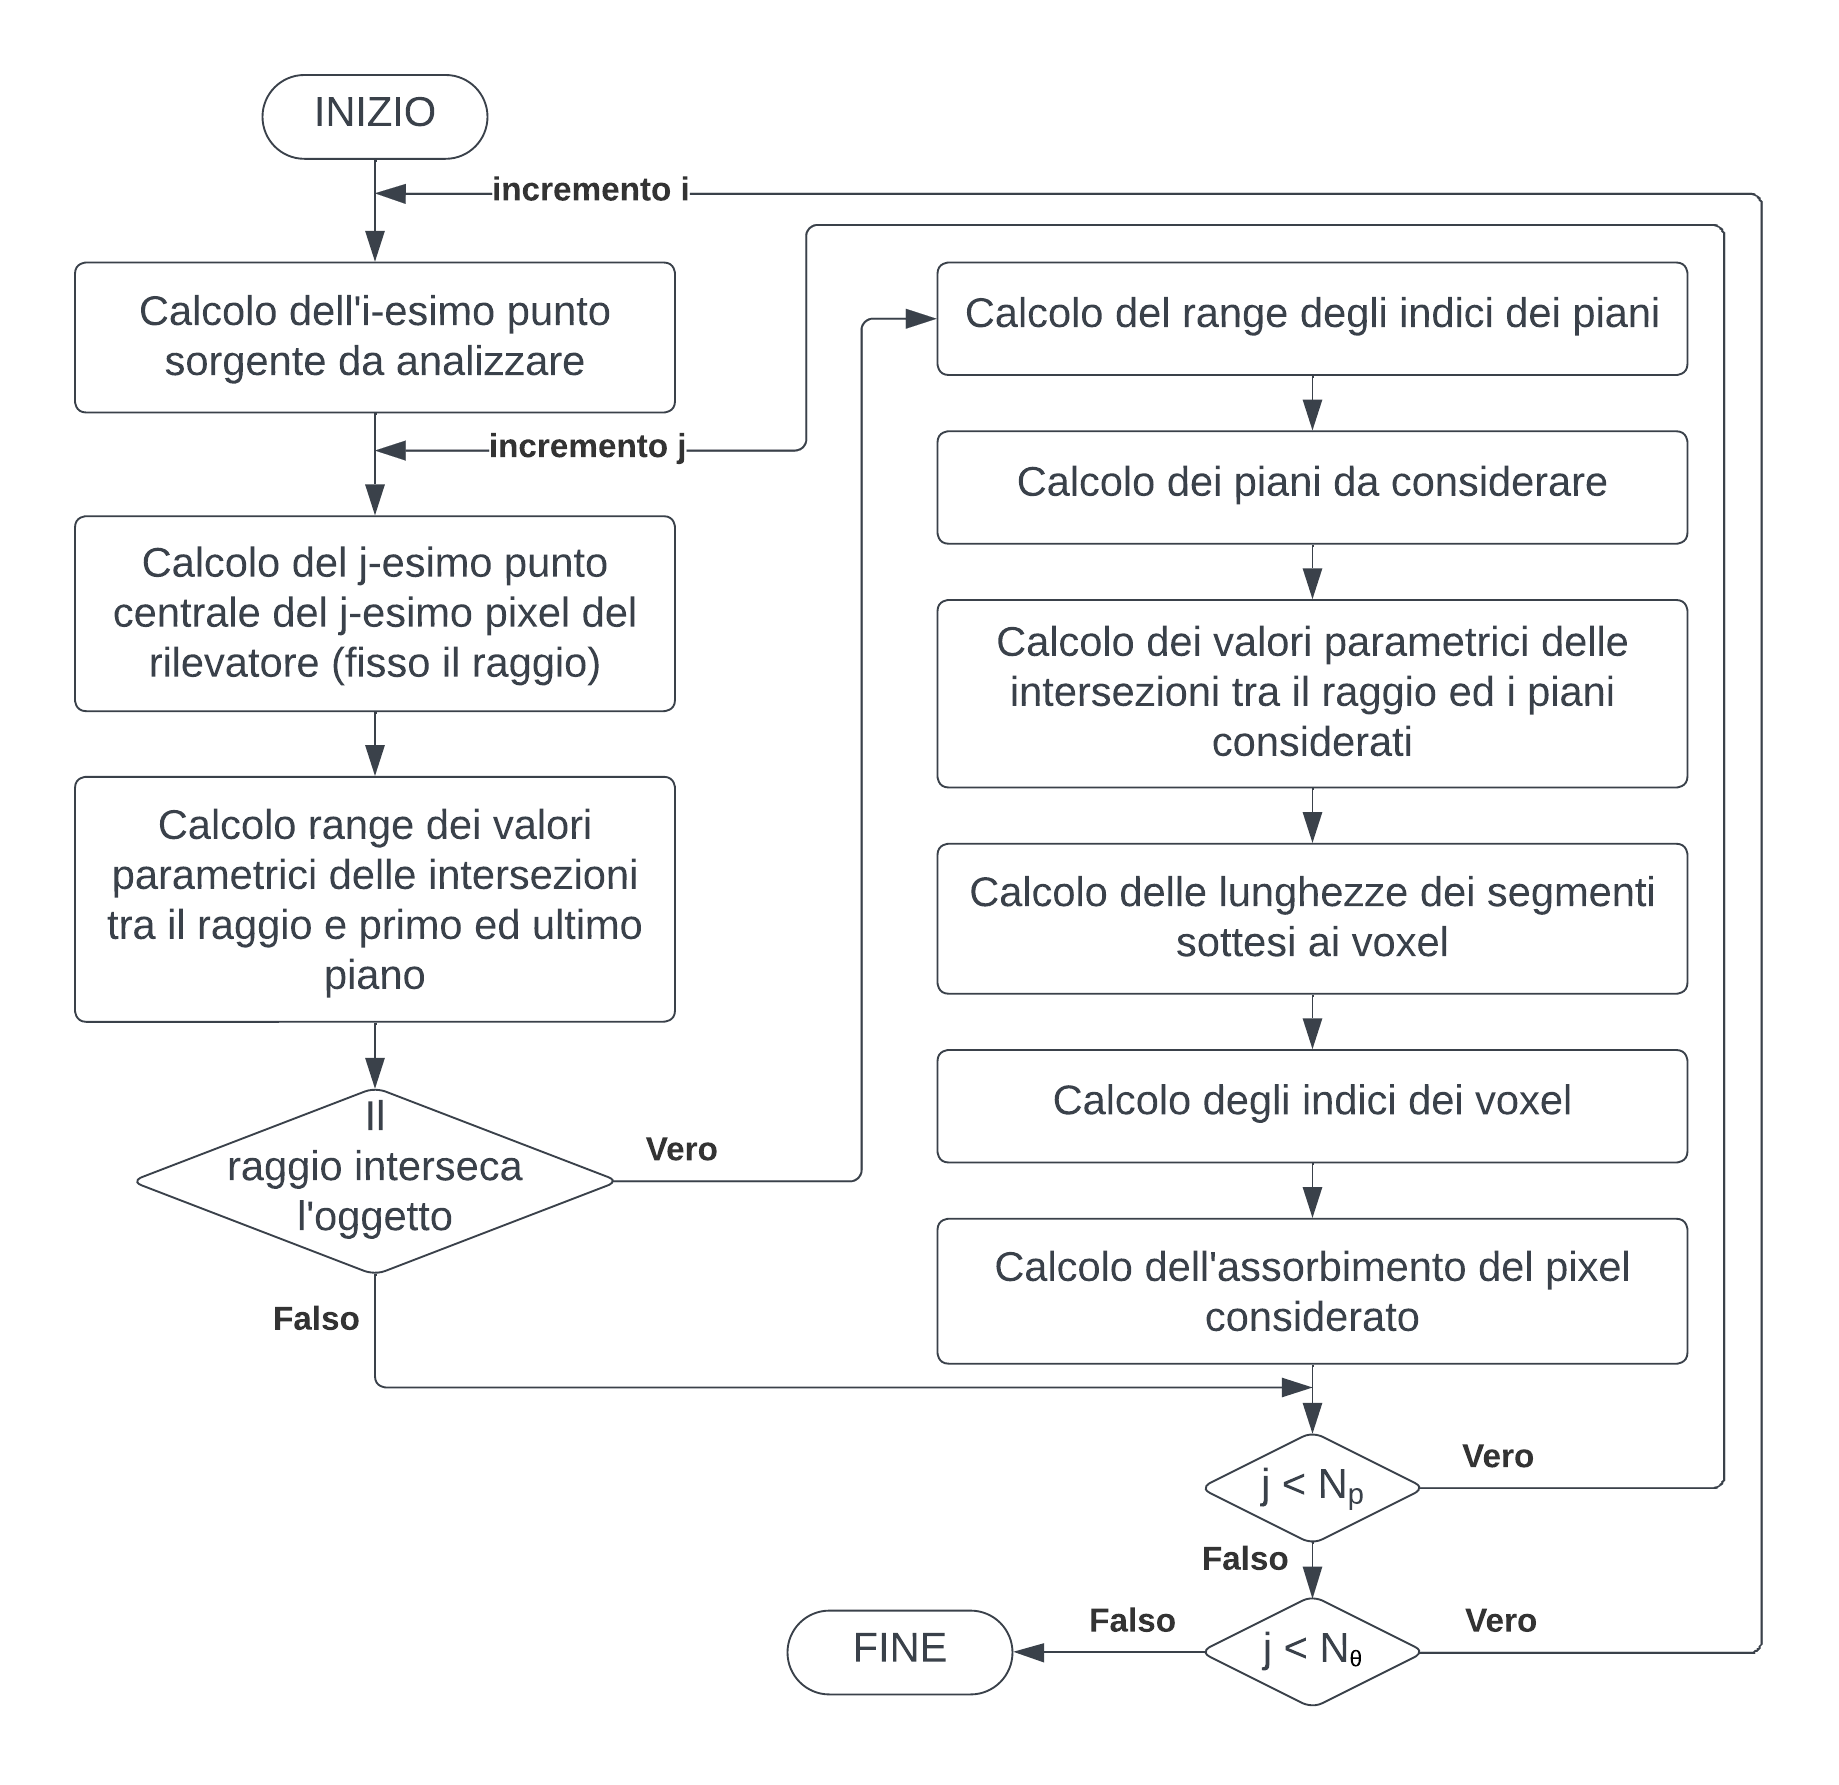
\includegraphics[width=\textwidth]{flowchart}
  \caption{Diagramma di flusso del calcolo delle proiezioni.}
  \label{fig:flowchart}
\end{figure}

In \autoref{fig:flowchart} è presentato il diagramma di flusso relativo ai punti 1-9 dell'algoritmo di calcolo delle proiezioni.

\subsection{Implementazione generale}

\subsubsection{1. Lettura input}

\begin{lstlisting}[language=CStyle, caption={Codice C per la lettura di \(f\).}, label={lst:vector_f_read}]
double *const f = (double *) malloc(sizeof(double) * gl_nVoxel[X] * yVoxels * gl_nVoxel[Z]);
...
for (unsigned short slice = 0; slice < gl_nVoxel[Y]; slice += yVoxels) {
  unsigned short nOfSlices;
  if (gl_nVoxel[Y] - slice < yVoxels) {
    nOfSlices = gl_nVoxel[Y] - slice;
  } else {
    nOfSlices = yVoxels;
  }
  fread(f, sizeof(double), (size_t) gl_nVoxel[X] * nOfSlices * gl_nVoxel[Z], inputFilePointer);
  ...
  computeProjections(...);
}
\end{lstlisting}

Il \autoref{lst:vector_f_read} mostra la gestione dell'array \(f\), che può costituire l'intero insieme di voxel o un suo
sottoinsieme.
La lettura dei dati viene quindi fatta considerando \lstinline{nOfSlices} voxel alla volta sull'asse \(y\), dove
\lstinline{yVoxels} è il numero di voxel considerati in una singola iterazione sull'asse \(y\).
Nella funzione \lstinline{computeProjections} sono sviluppati tutti i calcoli necessari per ottenere le proiezione.
Tutti i passi descritti successivamente sono svolti all'interno di tale funzione.

\subsubsection{2. Individuazione della prossima sorgente}

\begin{lstlisting}[language=CStyle, caption={Codice C per l'individuazione di un punto sorgente.}, label={lst:S_point}]
for (unsigned short positionIndex = 0; positionIndex < nTheta; positionIndex++) {
  const Point source = getSource(gl_sinTable, gl_cosTable, positionIndex);
  ... // Calcolo di ogni pixel del rilevatore
}
\end{lstlisting}

Il \autoref{lst:S_point} mostra come avviene il calcolo di ogni punto sorgente in base all'angolo di rotazione.
Il calcolo di ogni punto sorgente è ripetuto per ogni partizione considerata.
I dettagli della funzione \lstinline{getSource} non sono mostrati, il calcolo è lo stesso già presentato nella
\autoref{subsec:sources}.

\subsubsection{3. Individuazione del prossimo pixel del rilevatore}

\begin{lstlisting}[language=CStyle, caption={Codice C per l'individuazione di un pixel del rilevatore.}, label={lst:D_point}]
... // Per ogni sorgente
for (unsigned r = 0; r < nSidePixels; r++) {
  for (unsigned c = 0; c < nSidePixels; c++) {
    ...
    const Point pixel = getPixel(gl_sinTable, gl_cosTable, r, c, positionIndex);
    ... // Calcolo dell'assorbimento per il pixel considerato
  }
}
\end{lstlisting}

Il \autoref{lst:D_point} mostra come avviene il calcolo di ogni punto centrale di un pixel del rilevatore in base all'angolo di
rotazione.
I dettagli della funzione \lstinline{getPixel} non sono mostrati, il calcolo è lo stesso già presentato nella
\autoref{subsec:pixels}.

\subsubsection{4-9. Computazioni successive}

Le computazioni seguenti sono eseguite facendo riferimento all'algoritmo di Siddon \cite{Siddon1984}.

\subsection{Implementazione OpenMP}

L'implementazione per CPU proposta sfrutta il parallelismo OpenMP.

Il calcolo della soluzione, per motivi legati all'utilizzo di memoria RAM, viene fatto in partizioni, considerando di default un
numero massimo di \lstinline{100} voxel sull'asse \(y\).

Nella rielaborazione dell'implementazione di partenza è stata introdotta la possibilità di specificare il numero massimo di voxel
quando si lancia il programma da linea di comando, ignorando quindi il valore di default.

\subsubsection{Parallelizzazione}

In questo contesto, nonostante alcune modifiche, il modello di parallelizzazione è stato mantenuto invariato rispetto a quello del
codice originale.

\begin{lstlisting}[language=CStyle, caption={Codice C per il calcolo dell'assorbimento di un determinato pixel del rilevatore.}, label={lst:omp_D_point}]
... // Per ogni sorgente
#pragma omp parallel for collapse(2) schedule(dynamic) ...
for (unsigned r = 0; r < nSidePixels; r++) {
  for (unsigned c = 0; c < nSidePixels; c++) {
    ... // Calcolo dell'assorbimento per il pixel considerato
  }
}
\end{lstlisting}

Il \autoref{lst:omp_D_point} mostra le direttive OpenMP usate per parallelizzare il codice presentato nel \autoref{lst:D_point}.
Ogni processo OpenMP determina la posizione di un pixel del rilevatore e procede al calcolo dell'attenuazione che si verifica
quando il raggio attraversa la partizione dell'oggetto in esame.
La parallelizzazione viene eseguita considerando un carico di lavoro molto sbilanciato tra i diversi processi.
Infatti il numero di computazioni necessarie, per ogni raggio relativo ad una sorgente, potrebbe portare ad un carico di lavoro
molto disomogeneo.

È stata mantenuta la stessa versione di partenza che adottava un partizionamento a grana fine seguendo il paradigma master-worker,
in cui:
\begin{itemize}
  \item Partizionamento a grana fine: si riferisce a una suddivisione del lavoro in compiti molto piccoli, assegnati ai vari
        processi per massimizzare il parallelismo e bilanciare il carico.
        Nel nostro caso l'unità di parallelizzazione è il singolo valore fissato di \lstinline{r} e \mbox{\lstinline{c}.}
  \item Paradigma master-worker: è un modello di programmazione parallela in cui un processo master si occupa di assegnare i
        compiti ai processi worker.
        I worker eseguono i compiti assegnati e, una volta completato un task, passano immediatamente al successivo disponibile,
        seguendo l'ordine di completamento.
        Questo approccio consente una distribuzione dinamica ed efficiente del carico di lavoro, ottimizzando l'utilizzo delle
        risorse computazionali.
\end{itemize}

\subsection{Implementazione CUDA}

L'implementazione per GPU NVIDIA proposta sfrutta il parallelismo CUDA.

Analogamente alla versione OpenMP, la soluzione viene calcolata per partizioni, al fine di ottimizzare l'uso della memoria RAM.
Tuttavia, in questo caso, il numero massimo di voxel lungo l'asse \(y\) viene determinato dinamicamente mediante un algoritmo
euristico.
Questo algoritmo stima rapidamente la memoria occupata sulla GPU, fornendo un valore approssimativo che potrebbe non essere
necessariamente ottimale.

\begin{lstlisting}[language=CStyle, caption={Codice CUDA-C per il calcolo del numero massimo di voxel sull'asse \(y\).}, label={lst:cuda_y_max}]
size_t freeMem, totalMem;
cudaMemGetInfo(&freeMem, &totalMem);
freeMem -= (totalMem * 2 / 8);
unsigned tmp = gl_nVoxel[Y];
size_t size = sizeof(double) * gl_nVoxel[X] * tmp * gl_nVoxel[Z];
while (size > freeMem) {
  tmp = tmp * 5 / 8;
  if (tmp == 0) {
    fprintf(stderr,
      "The voxels Y size is too small respect to the other sizes:\n"
      "- N voxels X: %u.\n"
      "- N voxels Y: %u.\n"
      "- N voxels Z: %u.\n"
      "Total size reduced to the minimum possible is %lu Bytes!\n"
      "This is too much for this GPU with %lu Bytes of usable "
      "global memory (of %lu Bytes total)!\n",
      gl_nVoxel[X], gl_nVoxel[Y], gl_nVoxel[Z],
      size, freeMem, totalMem);
    termEnvironment();
    exit(EXIT_FAILURE);
  }
  size = sizeof(double) * gl_nVoxel[X] * tmp * gl_nVoxel[Z];
}
yVoxels = tmp;
\end{lstlisting}

Il \autoref{lst:cuda_y_max} mostra il funzionamento dell'algoritmo per il calcolo del numero massimo di voxel sull'asse \(y\) per
ogni partizione dell'input da considerare.
Dopo la sua individuazione il valore calcolato è assegnato a \mbox{\lstinline{yVoxels}.}

Anche in questo caso è stata introdotta la possibilità di specificare il numero massimo di voxel quando si lancia il programma da
linea di comando, ignorando quindi il valore generato dall'algoritmo euristico che agisce normalmente.

\subsubsection{Parallelizzazione}

Nelle discussioni seguenti, il termine host si riferirà all'esecuzione di codice seriale sulla CPU, mentre device indicherà
l'esecuzione di codice parallelo sulla GPU.

\begin{lstlisting}[language=CStyle, caption={Codice CUDA-C per la lettura di \(f\).}, label={lst:cuda_vector_f_read}]
double *const f = (double *) malloc(sizeof(double) * gl_nVoxel[X] * yVoxels * gl_nVoxel[Z]);
...
for (unsigned short slice = 0; slice < gl_nVoxel[Y]; slice += yVoxels) {
  unsigned short nOfSlices;
  if (gl_nVoxel[Y] - slice < yVoxels) {
    nOfSlices = gl_nVoxel[Y] - slice;
  } else {
    nOfSlices = yVoxels;
  }
  fread(f, sizeof(double), (size_t) gl_nVoxel[X] * nOfSlices * gl_nVoxel[Z], inputFilePointer);
  ...
  asyncComputeProjections(...);
}
\end{lstlisting}

Il \autoref{lst:cuda_vector_f_read}, equivalente del \autoref{lst:vector_f_read}, mostra come viene svolta la computazione
considerando partizioni dell'input.

In questo caso, a differenza di OpenMP, la funzione \lstinline{computeProjections} non viene invocata direttamente, bensì viene
chiamata un'altra funzione, \mbox{\lstinline{asyncComputeProjections}.}
Questa scelta è motivata dalla necessità di garantire coerenza con il tipo di computazione eseguita al suo interno.

Si noti che il prefisso \lstinline{async} nella funzione \mbox{\lstinline{asyncComputeProjections},} chiamata dall'host, indica
che l'esecuzione avviene in modo asincrono.
Così si permette alla CPU di leggere simultaneamente la prossima partizione dell'input, introducendo un ulteriore livello di
parallelismo tra le operazioni.

Tale meccanismo è reso possibile dalla separazione tra la memoria RAM della CPU e quella della GPU.
Di conseguenza, una volta copiati i dati di input nella RAM della GPU, la CPU può immediatamente sovrascrivere il buffer
contenente la partizione appena trasferita, subito dopo aver avviato il kernel in modalità asincrona.
Inoltre, nel caso in cui non ci siano più dati da essere letti allora il buffer di lettura può essere deallocato, in tal caso
l'host, inevitabilmente, attenderà il completamento del kernel per poter leggere i risultati ottenuti.

Questo approccio ha un impatto significativo sulla misurazione dei tempi di esecuzione: se il numero di iterazioni è elevato e la
durata dell'esecuzione del kernel non è inferiore a quella della lettura dell'input da file, è come se dal tempo totale di
esecuzione dei vari kernel (escluso l'ultimo) venisse sottratto il tempo di lettura da file.
In pratica, ciò si traduce in una riduzione complessiva dei tempi di esecuzione.

\begin{lstlisting}[language=CStyle, caption={Codice CUDA-C per il lancio del kernel.}, label={lst:cuda_launch_kernel}]
void asyncComputeProjections(...)
{
  // Si copia f dalla CPU nell'array corrispondente d_f sulla GPU
  cudaMemcpy(d_f, f, sizeF, cudaMemcpyHostToDevice);
  // Le dimensioni di griglia e blocco sono sempre le stesse
  static dim3 block(BLKDIM_STEP, BLKDIM_STEP);
  static dim3 grid((nSidePixels + BLKDIM_STEP - 1) / BLKDIM_STEP, (nSidePixels + BLKDIM_STEP - 1) / BLKDIM_STEP);
  // Il kernel viene lanciato in modo asincrono
  computeProjections<<<grid, block>>>(slice, nTheta, nSidePixels, d_f, d_g, isFirst);
}
\end{lstlisting}

Il \autoref{lst:cuda_launch_kernel} mostra l'inizializzazione del kernel CUDA.
Il kernel \mbox{\lstinline{computeProjections},} che si occupa del calcolo delle proiezioni, non è più eseguito nell'host,
ma nel device.
Quindi l'esecuzione dei passi 2-9 dell'algoritmo considerato, cioè del kernel, avviene in parallelo sul device.

\begin{lstlisting}[language=CStyle, caption={Codice CUDA-C del kernel.}, label={lst:cuda_kernel}]
__global__ void computeProjections(...)
{
  ...
  // r e c mappano ogni Thread su un singolo pixel del rilevatore
  const unsigned r = threadIdx.y + blockIdx.y * blockDim.y;
  const unsigned c = threadIdx.x + blockIdx.x * blockDim.x;

  // Gli eventuali Thread in eccesso non eseguono calcoli
  if (r < nSidePixels && c < nSidePixels) {
    // Calcolo dell'attenuazione di una coppia sorgente-pixel
    for (unsigned short positionIndex = 0; positionIndex < nTheta; positionIndex++) {
      const Point source = getSource(d_gl_sinTable, d_gl_cosTable, positionIndex);
      const Point pixel = getPixel(d_gl_sinTable, d_gl_cosTable, r, c, positionIndex);
      ... // Calcolo dell'assorbimento per il pixel considerato
    }
  }
}
\end{lstlisting}

Nel \autoref{lst:cuda_kernel} viene mostrato come ogni CUDA Thread determini la posizione di un pixel del rilevatore per procedere
al calcolo dell'attenuazione che si verifica quando il raggio attraversa la partizione dell'oggetto in esame.

Nel ciclo illustrato, ogni CUDA Thread analizza ciascuna sorgente in riferimento ad uno specifico pixel, che è lo stesso per ogni
iterazione sulle posizioni sorgente-rilevatore considerate.
Tale pixel è però ricalcolato di volta in volta perché traslato di un certo angolo.

Il vantaggio di questa soluzione è che viene creato un solo kernel per ogni partizione dell'input, garantendo così il numero
minimo possibile di esecuzioni.
Questo riduce al minimo l'overhead legato alla creazione dell'ambiente di esecuzione del kernel.
Inoltre, i dati necessari per il calcolo ad eccezione dell'input, che deve essere aggiornato per ogni partizione, vengono
trasferiti tra CPU e GPU una sola volta.

\section{Generazione output}

Il risultato dell'algoritmo di proiezione è l'array \(g\) di valori in virgola mobile, si faccia riferimento
all'\autoref{eq:law_lambert-beer_discrete}.
Tali valori vengono mappati su scala di grigi, facilitando la conversione in formato \lstinline{.pgm}, per poter poi essere
visualizzati come immagini, convertendoli in formati visualizzabili graficamente come \lstinline{.png}.

\begin{lstlisting}[language=CStyle, caption={Codice C per la mappatura dell'output in immagini.}, label={lst:outputs}]
double *const g = (double *) calloc(nSidePixels * nSidePixels * nTheta, sizeof(double));
... // Calcolo di g con OpenMP o CUDA
FILE *const outputFilePointer = fopen(outputFileName, "w");
if (!outputFilePointer) {
  fprintf(stderr, "Unable to open file '%s'!\n", outputFileName);
  free(g);
  return EXIT_FAILURE;
}
// Stampa un valore nell'intervallo [0-255]
fprintf(outputFilePointer, "P2\n%d %d\n255", nSidePixels, nSidePixels * nTheta);
for (unsigned short positionIndex = 0; positionIndex < nTheta; positionIndex++) {
  double angle = -(double) gl_angularTrajectory / 2 + (double) positionIndex * gl_positionsAngularDistance;
  fprintf(outputFilePointer, "\n#%lf", angle);
  for (unsigned i = 0; i < nSidePixels; i++) {
    fprintf(outputFilePointer, "\n");
    for (unsigned j = 0; j < nSidePixels; j++) {
      const unsigned pixelIndex = positionIndex * nSidePixels * nSidePixels + i * nSidePixels + j;
      int color = (g[pixelIndex] - gMinValue) * 255 / (gMaxValue - gMinValue);
      fprintf(outputFilePointer, "%d ", color);
    }
  }
}
fclose(outputFilePointer);
\end{lstlisting}

Il \autoref{lst:outputs} mostra come avviene la mappatura dei valori di \(g\) in un intervallo di valori 0-255 che individuano i
colori nero-bianco nella scala di grigi.

In un'immagine generata a partire dalla matrice di proiezione, i colori rappresentano visivamente i diversi livelli di
attenuazione.
Un raggio che attraversa una regione più densa del corpo subirà una maggiore attenuazione, risultando in una tonalità più chiara
(verso il bianco), mentre un raggio che attraversa una regione meno densa subirà una minore attenuazione, apparendo in una
tonalità più scura (verso il nero).

\begin{figure}[H]
  \centering
  \begin{subfigure}{\textwidth}
    \centering
    
\includegraphics[width=\textwidth]{Cube}
    \caption{\label{fig:projection_images_1} Cubo.}
  \end{subfigure}
  \begin{subfigure}{\textwidth}
    \centering
    
\includegraphics[width=\textwidth]{CubeWithSphericalHole}
    \caption{\label{fig:projection_images_2} Cubo con cavità sferica.}
  \end{subfigure}
  \begin{subfigure}{\textwidth}
    \centering
    
\includegraphics[width=\textwidth]{HalfSphere}
    \caption{\label{fig:projection_images_3} Semisfera.}
  \end{subfigure}
  \caption{\label{fig:projection_images} Immagini delle proiezioni.}
\end{figure}

La \autoref{fig:projection_images} mostra le immagini in formato \lstinline{.png} delle proiezioni ottenute eseguendo la versione
CUDA del programma.
Si ricorda che le immagini ottenute non sono fotografie tradizionali dell'oggetto scansionato, piuttosto sono una rappresentazione
della distribuzione di densità dell'oggetto scansionato.
In questo caso l'input processato è stato generato specificando \lstinline{2000} pixel per lato del detector, questo comporta che
ciascuna proiezione qui mostrata è costituita da \lstinline{2000x2000} pixel in scala di grigi.
In particolare le immagini riportate, lette da sinistra a destra, corrispondono alle proiezioni del rispettivo oggetto ottenute
considerando angoli di -45°, -30°, -15°, 0°, 15°, 30° e 45° in cui come asse polare si intende l'asse \(y\) e il senso orario di
rotazione delle sorgenti.
Le proiezioni sono state calcolate considerando come angoli di posizionamento della sorgente rispetto all traiettoria circolare
\(\theta = 90^\circ\) e \(\alpha = 15^\circ\), rivedi \autoref{fig:CT_polar_coordinates_source}.

È importante inoltre considerare che, a causa delle differenze nelle architetture hardware di CPU e GPU, unitamente al fatto che
l'ordine dei l'ordine dei calcoli in virgola mobile eseguiti in OpenMP e CUDA può variare, i risultati ottenuti non saranno
esattamente identici.
Per confrontare i risultati delle due versioni del programma e verificarne la correttezza, si possono adottare due approcci:
\begin{itemize}
  \item Comparare direttamente le versioni binarie dei risultati, scrivendo la matrice \(g\) su file.
        Questo è il metodo più accurato.
  \item Comparare le versioni \lstinline{.pgm} dei risultati, dove gg viene mappata da una matrice di valori in virgola mobile a
        un'altra di valori nell'intervallo 0-255.
        Questo metodo è meno accurato.
  \item Comparare le versioni \lstinline{.png} dei risultati ad occhio.
        Questo metodo è il meno accurato.
\end{itemize}
Per i risultati generati, oltre alla verifica visiva, cioè il terzo metodo, come conferma è stato utilizzato il secondo metodo.
Su Linux, questo confronto può essere effettuato tramite il comando:

\lstinline{compare -metric RMSE PGM1 PGM2 OUTPUT}

dove:
\begin{itemize}
  \item \lstinline{PGM1} va rimpiazzato con il percorso del primo file in formato \lstinline{.pgm} da considerare.
  \item \lstinline{PGM2} va rimpiazzato con il percorso del secondo file in formato \lstinline{.pgm} da considerare.
  \item \lstinline{OUTPUT} va rimpiazzato con il percorso del file in cui verranno scritte le differenze tra i due file
        considerati.
\end{itemize}

Si deve inoltre considerare che se la metrica RMSE (Root Mean Square Error) ottenuta è un valore sotto a \lstinline{1000}
allora i due risultati possono essere considerati molto simili.

\chapter{Valutazione delle prestazioni}

Nella valutazione delle prestazioni per l'implementazioni CUDA trattata in questo progetto di tesi, le metriche di analisi
considerate sono il tempo di esecuzione, il throughput e lo speedup rispetto alla versione OpenMP.

Si inizierà analizzando la complessità computazionale dell'algoritmo implementato, per poi presentare le statistiche ottenute dai
test pratici eseguiti su un server.

Sia per OpenMP che per CUDA è stata utilizzata la versione di default dei programmi.
Per OpenMP si considera un numero massimo di \lstinline{100} voxel sull'asse \(y\), mentre per CUDA questo valore è determinato
dall'algoritmo euristico descritto in precedenza.

\section{Statistiche}

Prima di analizzare i risultati ottenuti è utile individuare la complessità computazionale dell'algoritmo considerato.
Il limite superiore del tempo di esecuzione dell'algoritmo viene già individuato nella tesi di Colletta \cite{Colletta2024}.
Tale complessità computazionale è qui riproposta:

\begin{equation} \label{eq:computational_complexity}
  O(N_\theta \cdot N_{pixel}^2 \cdot (N_x + N_y + N_z))
\end{equation}

dove:
\begin{itemize}
  \item \(O\) detta o-grande, indica che si tratta di un limite superiore del tempo di esecuzione, relativo al caso in cui un
        raggio interseca tutti i piani.
  \item \(N_\theta\) è il numero di proiezioni calcolate, cioè il numero di posizioni della sorgente considerate.
  \item \(N_{pixel}\) è il numero di unità di misurazione per lato del rilevatore.
  \item \(N_x\) è il numero di voxel lungo l'asse \(x\).
  \item \(N_y\) è il numero di voxel lungo l'asse \(y\).
  \item \(N_z\) è il numero di voxel lungo l'asse \(z\).
\end{itemize}

Il server considerato nei test riportati successivamente è l'\mbox{\lstinline{isi-raptor03.csr.unibo.it}.}
La CPU del server è un \lstinline{Intel(R) Xeon(R) CPU E5-2603 v4 @ 1.70GHz} con 12 core fisici e 12 core logici (quindi senza
Hyper-Threading).
La scheda madre è dotata di 64 GB di RAM.
La GPU usata nel server è una \mbox{\lstinline{NVIDIA GeForce GTX 1070}.}
La scheda grafica è dotata di 8 GB di RAM.

Gli input considerati sono i file \lstinline|CubeWithSphericalHole{400-1500}.dat|, cioè del tipo: cubo con cavità sferica.
Il numero di pixel per lato della matrice rilevatore varia da \lstinline{400} a \lstinline{1500} con intervalli di \lstinline{100}
pixel tra un input ed il successivo, per un totale di 12 input diversi.

\begin{table}[H]
  \centering
  \begin{tblr}{
      colspec={*{4}{Q[c]}},
      width=\textwidth,
      row{odd}={gray!15},
      row{even}={white},
      row{1}={bg=gray!90,fg=white},
      colsep=4pt
    }
      \textbf{Iterazione} & $\bm{N_\theta}$ & $\bm{N_{pixel}}$ & $\bm{N_x}$ & $\bm{N_y}$ & $\bm{N_z}$ \\
      \textbf{1} & 7 & 400 & \SetCell[c=3]{c} 168 \\
      \textbf{2} & 7 & 500 & \SetCell[c=3]{c} 210 \\
      \textbf{3} & 7 & 600 & \SetCell[c=3]{c} 252 \\
      \textbf{4} & 7 & 700 & \SetCell[c=3]{c} 294 \\
      \textbf{5} & 7 & 800 & \SetCell[c=3]{c} 336 \\
      \textbf{6} & 7 & 900 & \SetCell[c=3]{c} 378 \\
      \textbf{7} & 7 & 1000 & \SetCell[c=3]{c} 420 \\
      \textbf{8} & 7 & 1100 & \SetCell[c=3]{c} 462 \\
      \textbf{9} & 7 & 1200 & \SetCell[c=3]{c} 504 \\
      \textbf{10} & 7 & 1300 & \SetCell[c=3]{c} 546 \\
      \textbf{11} & 7 & 1400 & \SetCell[c=3]{c} 588 \\
      \textbf{12} & 7 & 1500 & \SetCell[c=3]{c} 630 \\
  \end{tblr}
  \caption{\label{tab:cuda_it_sizes} Dimensioni del problema per ogni iterazione considerata.}
\end{table}

La \autoref{tab:cuda_it_sizes} mostra quali sono le dimensioni del problema.
\(N_\theta\) è costante perché identificato dagli angoli fissati \(\theta = 90^\circ\) e \(\alpha = 15^\circ\).
Il numero di voxel sui vari assi \(N_x\), \(N_y\) e \(N_z\) sono uguali perché viene considerato un oggetto cubico.
Tale valore del numero di voxel per asse viene calcolato dal generatore di input in base al numero di pixel per lato del
rilevatore scelti per ogni iterazione in modo empirico in base all'hardware a disposizione, \(N_{pixel}\).

\subsection{Tempo di esecuzione}

Il tempo di esecuzione potrebbe essere semplicemente considerato come il tempo totale impiegato dal programma per completare
l'elaborazione.
Tuttavia, questo includerebbe anche i tempi di lettura dell'input e di scrittura dell'output, influenzando significativamente la
misurazione.
Per questo motivo, nel seguito verrà considerato il tempo di esecuzione dato da:
\begin{itemize}
  \item Allocazione dati: per la CPU semplicemente l'allocazione delle strutture dati e la loro opportuna inizializzazione, per la
        GPU anche il trasferimento dalla RAM dell'host a quella del device.
  \item Esecuzione dei calcoli dei valori di attenuazione per ogni chiamata alla funzione OpenMP \lstinline{computeProjections} o
        a quella CUDA \mbox{\lstinline{asyncComputeProjections}.}
  \item Deallocazione dati: per la CPU semplicemente la deallocazione delle strutture dati, per la GPU anche il trasferimento
        dalla RAM del device a quella dell'host.
\end{itemize}
Non verranno considerati:
\begin{itemize}
  \item Tempo di esecuzione della lettura da file dell'input, perché le operazioni sono le stesse in entrambe le versioni.
  \item Tempo di esecuzione della scrittura su file dell'output, perché anche se il risultato delle due versioni è leggermente
        diverso a causa dei calcoli in virgola mobile, le operazioni eseguite sono le stesse.
\end{itemize}

\begin{figure}[H]
  \centering
    \begin{tikzpicture}[scale=0.9]
      \begin{axis}[
        title={Tempi di esecuzione},
        xlabel={Numero di pixel per lato del rilevatore},
        ylabel={Tempo di esecuzione (s)},
        xlabel style={yshift=-10pt},
        xtick=data,
        symbolic x coords={400, 500, 600, 700, 800, 900, 1000, 1100, 1200, 1300, 1400, 1500},
        x tick label style={rotate=45, anchor=east},
        ymin=0, ymax=30,
        ytick={0,2,4,6,8,10,12,14,16,18,20,22,24,26,28,30},
        legend pos=north west,
        grid=both
      ]
        % OpenMP
        \addplot[
          thick,
          color=blue,
          mark=*,
        ]
          coordinates {
            (400, 0.55) (500, 1.18) (600, 1.88)
            (700, 2.73) (800, 4.33) (900, 6.05)
            (1000, 8.56) (1100, 10.92) (1200, 15.21)
            (1300, 17.97) (1400, 21.97) (1500, 27.82)
          };
        \addlegendentry{\small{OpenMP}}
        % CUDA
        \addplot[
          thick,
          color=green,
          mark=*,
        ]
          coordinates {
            (400, 0.37) (500, 0.42) (600, 0.54)
            (700, 0.67) (800, 0.83) (900, 1.05)
            (1000, 1.30) (1100, 1.62) (1200, 2.02)
            (1300, 2.58) (1400, 3.13) (1500, 3.66)
          };
        \addlegendentry{\small{CUDA}}
      \end{axis}
    \end{tikzpicture}
    \caption{\label{fig:cuda_wall_clock_time} Tempi di esecuzione di CUDA ed OpenMP a confronto.}
\end{figure}

La \autoref{fig:cuda_wall_clock_time} mostra i tempi di esecuzione a confronto per OpenMP e CUDA.
Come si può notare i tempi di esecuzione della versione CUDA sono fino alle 7 volte inferiori rispetto a quelli della versione
OpenMP.

\subsection{Throughput}

Il throughput, è il numero di operazioni al secondo in funzione della dimensione dell'input.
La dimensione dell'input è approssimata con il lavoro svolto dall'algoritmo, vedi l'\autoref{eq:computational_complexity}.

\begin{figure}[H]
  \centering
    \begin{tikzpicture}[scale=0.9]
      \begin{axis}[
        title={Throughput},
        xlabel={Numero di pixel per lato del rilevatore},
        ylabel={Operazioni (Gops/s)},
        xlabel style={yshift=-10pt},
        xtick=data,
        symbolic x coords={400, 500, 600, 700, 800, 900, 1000, 1100, 1200, 1300, 1400, 1500},
        x tick label style={rotate=45, anchor=east},
        ymin=0, ymax=9,
        scaled y ticks=false,
        ytick={0,1,2,3,4,5,6,7,8,9},
        legend pos=north west,
        grid=both
      ]
        % OpenMP
        \addplot[
          thick,
          color=orange,
          mark=*,
        ]
          coordinates {
            (400, 1.03) (500, 0.94) (600, 1.01)
            (700, 1.11) (800, 1.04) (900, 1.06)
            (1000, 1.03) (1100, 1.08) (1200, 1.00)
            (1300, 1.08) (1400, 1.10) (1500, 1.07)
        };
        \addlegendentry{\small{OpenMP}}
        % CUDA
        \addplot[
          thick,
          color=pink,
          mark=*,
        ]
          coordinates {
            (400, 1.55) (500, 2.61) (600, 3.50)
            (700, 4.55) (800, 5.43) (900, 6.15)
            (1000, 6.77) (1100, 7.26) (1200, 7.54)
            (1300, 7.51) (1400, 7.74) (1500, 8.13)
        };
        \addlegendentry{\small{CUDA}}
      \end{axis}
    \end{tikzpicture}
    \caption{\label{fig:cuda_throughput} Throughput di CUDA ed OpenMP a confronto.}
\end{figure}

Il throughput è calcolato come \(\frac{Numero\ di\ operazioni}{Tempo\ di\ esecuzione\ (s)}\).
Per stimare il limite superiore del numero di operazioni al secondo svolte dai programmi sono stati utilizzati i dati riportati
nella \autoref{tab:cuda_it_sizes}, i risultati sono osservabili nella \autoref{fig:cuda_throughput}.
Tale numero di istruzioni è approssimato a miliardi di operazioni per secondo.
In questo caso, il numero di operazioni al secondo per CUDA arriva fino a 8x rispetto a quello della versione OpenMP.

\subsection{Speedup}

Lo speedup di CUDA è inteso come il confronto dei tempi di esecuzione della versione CUDA rispetto a quella OpenMP.
Indica quanto l'implementazione per GPU è mediamente più veloce rispetto a quella per la CPU, al variare della dimensione
dell'input.

\begin{figure}[H]
  \centering
    \begin{tikzpicture}[scale=0.8]
        \begin{axis}[
          x=1cm,
          width=12cm, height=8cm,
          title={Speedup},
          xlabel={Numero di pixel per lato del rilevatore},
          ylabel={Speedup},
          xlabel style={yshift=-10pt},
          xtick=data,
          symbolic x coords={400, 500, 600, 700, 800, 900, 1000, 1100, 1200, 1300, 1400, 1500},
          x tick label style={rotate=45, anchor=east},
          ymin=0, ymax=8,
          legend pos=north west,
          bar width=0.7cm,
          nodes near coords,
          grid=none
        ]
          \addplot[ybar, fill=cyan] coordinates {
            (400, 1.50) (500, 2.79) (600, 3.46)
            (700, 4.10) (800, 5.21) (900, 5.79)
            (1000, 6.57) (1100, 6.75) (1200, 7.53)
            (1300, 6.97) (1400, 7.03) (1500, 7.60)
          };
        \end{axis}
    \end{tikzpicture}
    \caption{\label{fig:cuda_speedup} Accelerazione di CUDA rispetto ad OpenMP.}
\end{figure}

La \autoref{fig:cuda_speedup} mostra le performance della versione CUDA rispetto a quella OpenMP.
Per input piccoli, l'accelerazione della versione CUDA è limitata, mentre cresce con la dimensione, stabilizzandosi intorno a 6x,
con un picco di 7.6x in un caso favorevole.

\appendix

\chapter{Conclusioni}

\dots

\label{mylastpage}
\printbibliography % Print the bibliography
\thispagestyle{empty} % Avoids numbering on the first bibliography page
\pagestyle{empty} % Avoids numbering on all bibliography pages after the first

\end{document}
